\documentclass[titlepage, a4paper, 11pt]{article}


\usepackage[english]{babel}

\usepackage[a4paper, left=1in,right=1in,top=1in,bottom=1in,]{geometry}

% Useful packages
\usepackage{amsmath}
\usepackage{subcaption}
\usepackage{float}
\usepackage{biblatex}
\addbibresource{sample.bib}
\usepackage{graphicx}
\graphicspath{ {./images/} }
\usepackage[]{hyperref}
\usepackage{multirow}

\setlength{\parindent}{0pt}



\usepackage{caption}
\captionsetup{font=small}

\begin{document}
\begin{titlepage}
	\begin{center}
		\vspace*{1cm}
        \hline
        \vspace{0.4cm}
		\textbf{\Huge Fluid Mechanics Project Report}
		\vspace{0.4cm}
		\hline

		\vspace{2cm}
		\textbf{\huge{Fluid Flow through a Valvular Conduit }}

		\vspace{5cm}
		
		
        
\includegraphics[width=0.7\textwidth]{images/koclogo.png}
        
        
        \vfill
        
		\Large{Deniz Erdogan - 69572}

        January 10, 2022	

		\vspace{0.8cm}


	\end{center}
\end{titlepage}

\tableofcontents
\newpage
\listoffigures
\listoftables
\newpage

%%%%%%%%%%%%%%%%%%%% Introduction %%%%%%%%%%%%%%%%%%%%
\section{Introduction}
This project focuses on the behavior of a no-moving-parts check valve designed by Nikola Tesla, also known as Tesla valve under different conditions and configurations. Particularly, we will be focusing on incompressible viscous flow through a valvular conduit. ANSYS Fluent will be used as the means of simulation. \\

This valvular conduit allows the fluid flow to pass through very easily in one direction while resisting significantly to flows in the other direction. This feature of the geometry allows it to be used in various applications such as flow control, mixing fluid streams and microfluidic applications. The design is aimed to cause higher pressure drops in one direction than the other. The ratio of the pressure drops in two directions is called diodicity and is calculated as follows:
\begin{equation}
    Di = \frac{\Delta p_r}{\Delta p_f}
\end{equation}

Also, throughout this project the studies of Truong et al \cite{truong} and Nguyen et al \cite{nguyen_abouezzi_ristroph_2021} will be referenced for optimization information.\\

In the first task forward flow for laminar flow is analyzed and the development of the boundary layer is shown using data and velocity profiles from different cross sections Later on, the solution is validated by comparing it with an analytical solution known as the \textbf{Couette solution}. This is of course valid when the flow is fully developed. \\

Following this, task two focuses on the optimization of the straight line segment on the valvular conduit. A relation between the Reynolds number and optimum length will be derived by fitting curves to our data and will be compared with the equations provided by the other studies. Simulations will be conducted for different Reynolds numbers, lengths and directions of which the diodicities will be calculated for each case and plotted. Later on, using the optimized values, a new simulation will be conducted to test the diodicity. \\

For the last part, unlike the work done before, a three dimensional analysis will be conducted using two different turbulence models, them being $k - \epsilon$ and $k - \omega$ models. The optimal design parameters will be used that were derived from previous tasks. The discrepancies between the two models will be compared and discussed along with the diodicity value obtained in this step. \\

\textbf{\textit{Keywords:}} CFD, internal flow, Tesla valve.


\newpage

%%%%%%%%%%%%%%%%%%%% Problem Descriptions %%%%%%%%%%%%%%%%%%%%
\section{Problem Descriptions}

\subsection{Task 1: Initial Observations on the Valve}
\label{sec:task1}

In this section, first simulations will be done on the valvular conduit. As the first ste, the sketch of the valve must be constructed. For the dimensional parameters, the optimum values of $\alpha$, $\beta$ and R are chosen so that the inner circular arc is tangent to the x-axis. A sample sketch for this geometry can be seen on Figure \ref{fig:sampsketch}.

\begin{figure}[H]
    \centering
    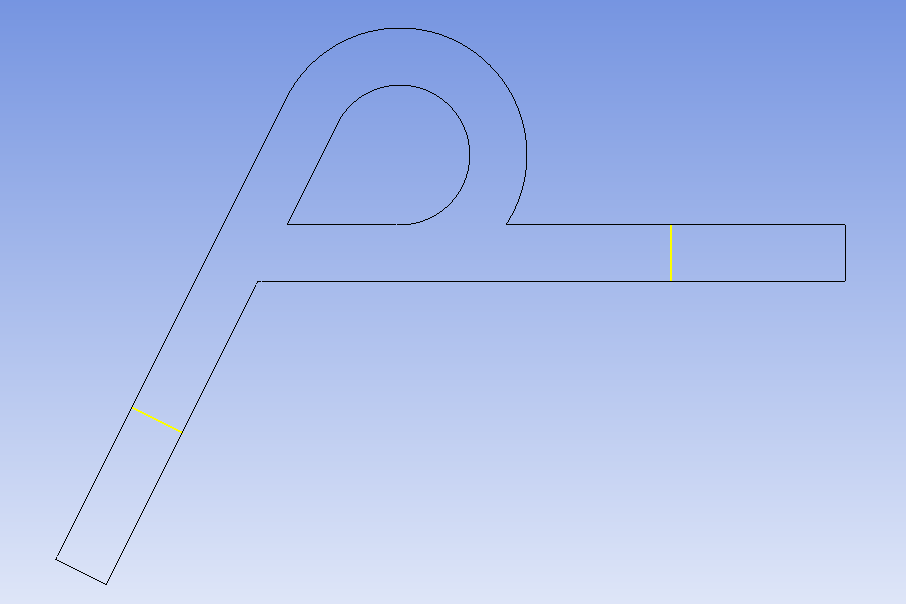
\includegraphics[width=.6\textwidth]{images/task1/data_locations.png}
    \caption{Sample Sketch}
    \label{fig:sampsketch}
\end{figure}

For this geometry, the straight line segment is selected to be 200mm long and Re is chosen to be 181. To obtain that value the velocity and material properties as manipulated as follows:
\begin{itemize}
    \item $\mu = 4.6.10^{-4}$Pa.s
    \item $\rho = 1000 kg/m^{3}$
    \item $D = 100$mm
    \item $V = 0.0008326$m/s
\end{itemize}

For the boundary conditions, no-slip on channel walls and uniform inlet velocity are set. This task only tests the forward flow throughout the inlet. To achieve this, the inlet is selected to be the end of the horizontal segment at the right-hand side of the sketch. To observe the grid-independence of the solution, two different mesh sizes are used, them being $6.10^{-3}$ and $6.10^{-3}$ meters with adaptive meshing. In order to prove that grid convergence is achieved, velocity profile of the fluid halfway through the inlet segment and outlet segment is plotted between two mesh sizes. As can be seen from Figure \ref{fig:mesh_comp}, the results does not change considerably with reducing mesh size. From this, a mesh size of $3.10^{-3}$m will be used in this project unless stated otherwise. 

\begin{figure}[H]
 \centering
\begin{subfigure}{.45\textwidth}
  \centering
  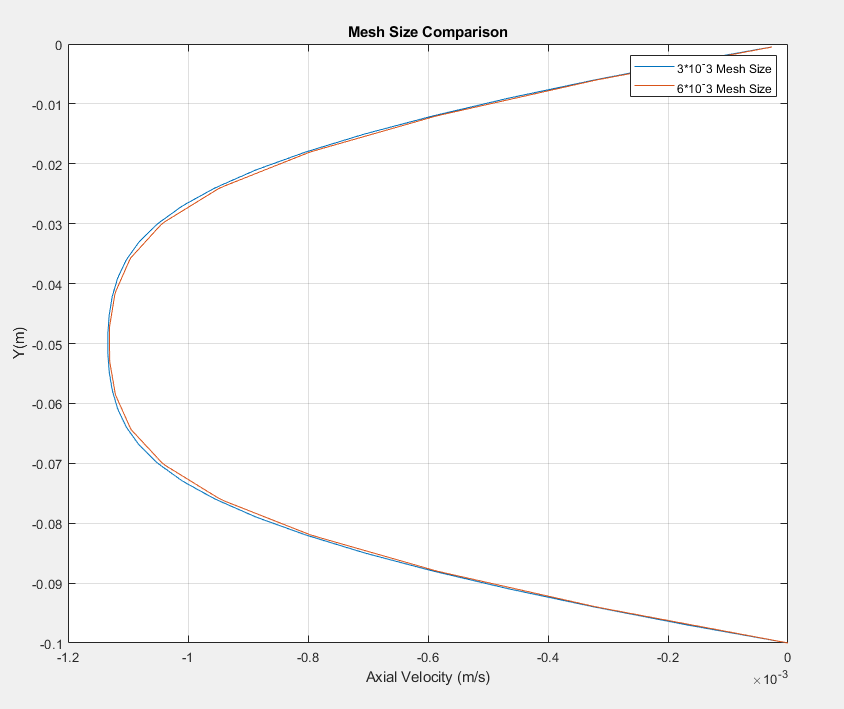
\includegraphics[width=.87\linewidth]{images/task1/3vs6mesh.png}
  \caption{Profile at the inlet}
  \label{fig:x_d_norm}
\end{subfigure}%
~
\begin{subfigure}{.45\textwidth}
  \centering
  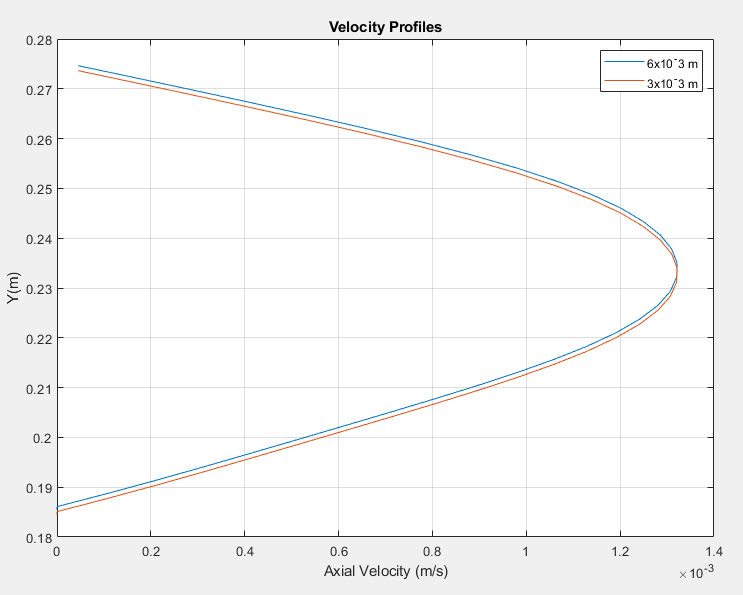
\includegraphics[width=.9\linewidth]{images/task1/outlet_mesh_comparison.png}
  \caption{Profile at the outlet}
  \label{fig:x_d_norm_actual}
\end{subfigure}
~
\caption{Mesh Size Comparison}
\label{fig:mesh_comp}
\end{figure}

\subsection{Task 2: Investigation on the Effect of the Partition Straight Segment}
\label{sec:task2_desc}

This section revolves around observing and commenting on the effects of the partition straight segment, denoted $L$, on the pressure drop caused by the valve for different values of Reynolds number. Following this,  a correlation is to be found for the optimum straight segment length $L$,
normalized by the channel width $W$ as a function of the Reynolds number. \\

In their work, Truong et al \cite{truong}, have made a similar analysis and optimization on $\alpha$, of which we are using in this simulation to obtain optimal drop. However, in our case, we will be applying the same principles to $L$, which then will be tested thoroughly. 18 different simulations will be conducted for 3 different $L/W$ ratios, adjusting $L$ to be 200, 400 and 600mm while also changing the Reynolds Number for 3 different values and doing so in each direction for each configuration. The grid converged setup from Task-1 is used for these iterations. \\

$\alpha_{opt}$ will be used as given in the equation of Truong and Nam Trung \cite{truong} and pressure drops are measured by checking the pressure values at the center of the inlets and outlets for all cases, accounting for the switch of boundaries in each step.\\

Following our modeling of the system, simulations for Re = 724 in both flow directions with the corresponding $L_{opt}$, $\alpha_{opt}$, R and $\beta$ dimensions for the geometry will be conducted. Also, the same mesh size will be used as the tasks before. The new diodicity will be examined along with velocity plots, pressure plots and streamlines.

\subsection{Task 3: Turbulence Analysis in 3D for the Optimized Geometry}
\label{sec:task3}

In this part of the project, the valvular conduit is examined in 3 dimensions using the optimal geometric dimensions including the optimum $L$ value found from \ref{sec:task2results}. The Reynolds number for this setup is set to be $10^4$ while the optimizations are done according to Re = 724. Simulations have been conducted in both directions using both the $k - \epsilon$ and $k - \omega$ solvers. To obtain the Reynolds number of $10^4$, the parameters are set as follows:
\begin{itemize}
    \item $\rho = 5000$kg/$m^3$
    \item V = 0.02 m/s
    \item $\mu = 10^-3$Pa.s
\end{itemize}

Following this, using the pressure contours and streamline plots for both directions, the diodicities are calculated and the effects are discussed. 





%%%%%%%%%%%%%%%%%%%% Results and Discussion %%%%%%%%%%%%%%%%%%%%%
\section{Results and Discussion}
\subsection{Task 1 Results}
\label{sec:task1results}
\subsubsection{Geometry and Mesh}
As described in \ref{sec:task1}, simulations have been conducted for the finest mesh size depicted there. Also, after each simulation, the residuals are tracked and checked for convergence. Only then will the results be meaningful in terms of steady-state conditions. For observation, the velocity profiles at the inlet and the outlet are plotted and can be seen from Figure \ref{fig:in_out_comparison}. The velocity profiles are taken from the cross sections that lie on the middle of the straight line segments both at the inlet and outlet. As expected, we see a parabolic shape in both cases with the maximum occurring at the center of the cross section. Also, the mesh used for this experiment can be seen on Figure \ref{fig:mesh}. 

\begin{figure}[H]
    \centering
    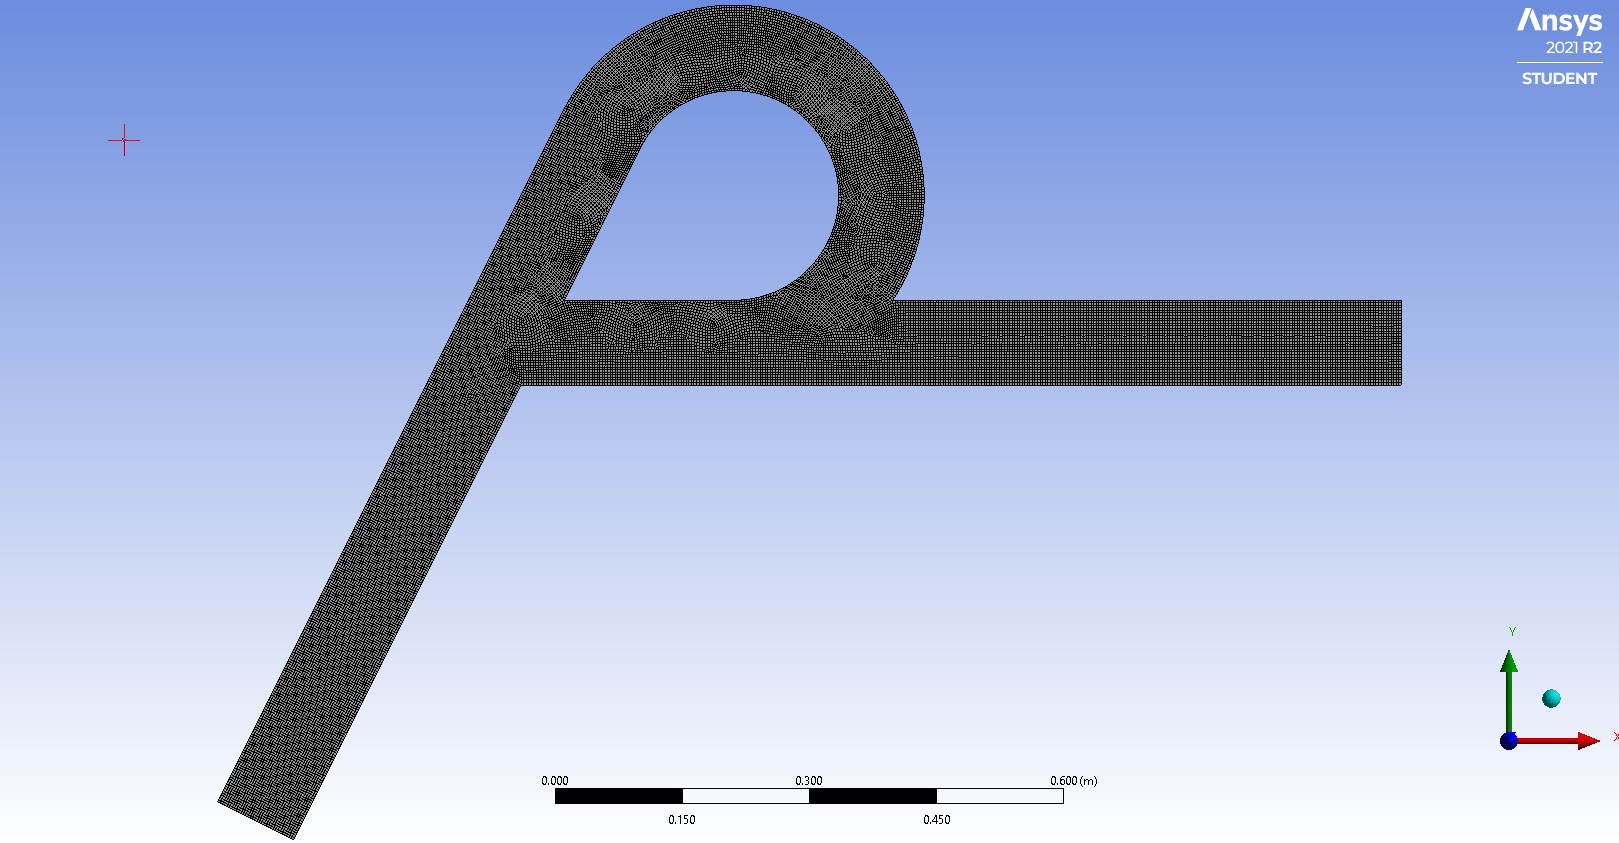
\includegraphics[width=.7\textwidth]{images/task1/3_mesh.png}
    \caption{Sample Mesh}
    \label{fig:mesh}
\end{figure}


\begin{figure}[H]
    \centering
    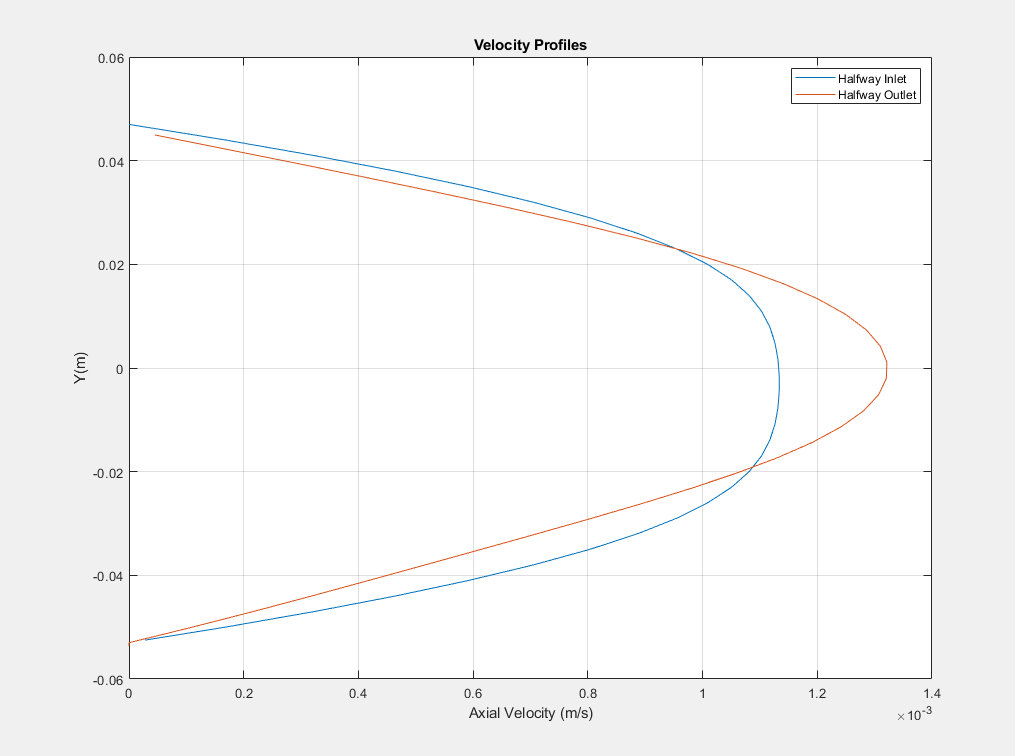
\includegraphics[width=.7\textwidth]{images/task1/3inlet_vs_outlet.png}
    \caption{Comparison of Inlets and Outlets}
    \label{fig:in_out_comparison}
\end{figure}

\subsubsection{Validation}
Further on, to validate our results our computational solutions will be compared with the analytical solutions. For this case, the Couette solution can be applied. The equation for this solution is as follows:
\begin{equation}
    u = 6 * V_{ave} * \Big( \frac{y}{w} - \frac{y^2}{w^2}\Big)
\end{equation}


For validation, the equation is plotted against the ANSYS data we have resulted in, Figure \ref{fig:couette} shows this comparison. As expected, our results agree greatly with the analytical results. For this plot, the ANSYS data are taken from cross sections 75\% into the straight line segments both for the inlet and outlet sections.

\begin{figure}[H]
    \centering
    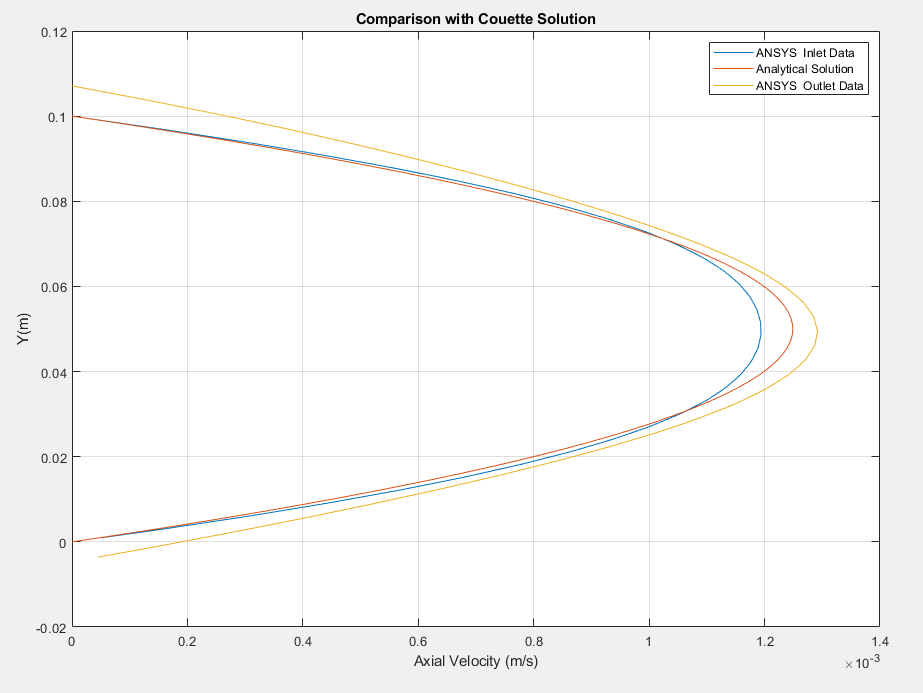
\includegraphics[width=.7\textwidth]{images/task1/couette.png}
    \caption{CFD vs Analytical}
    \label{fig:couette}
\end{figure}


Moreover, various velocity profiles inside are plotted over to demonstrate the development of the boundary layer. Figure \ref{fig:development} shows this plot. The distances from the inlet of those cross sections are as follows:
\begin{itemize}
    \item 10mm
    \item 40mm
    \item 150mm
    \item 225mm
\end{itemize}



\begin{figure}[H]
    \centering
    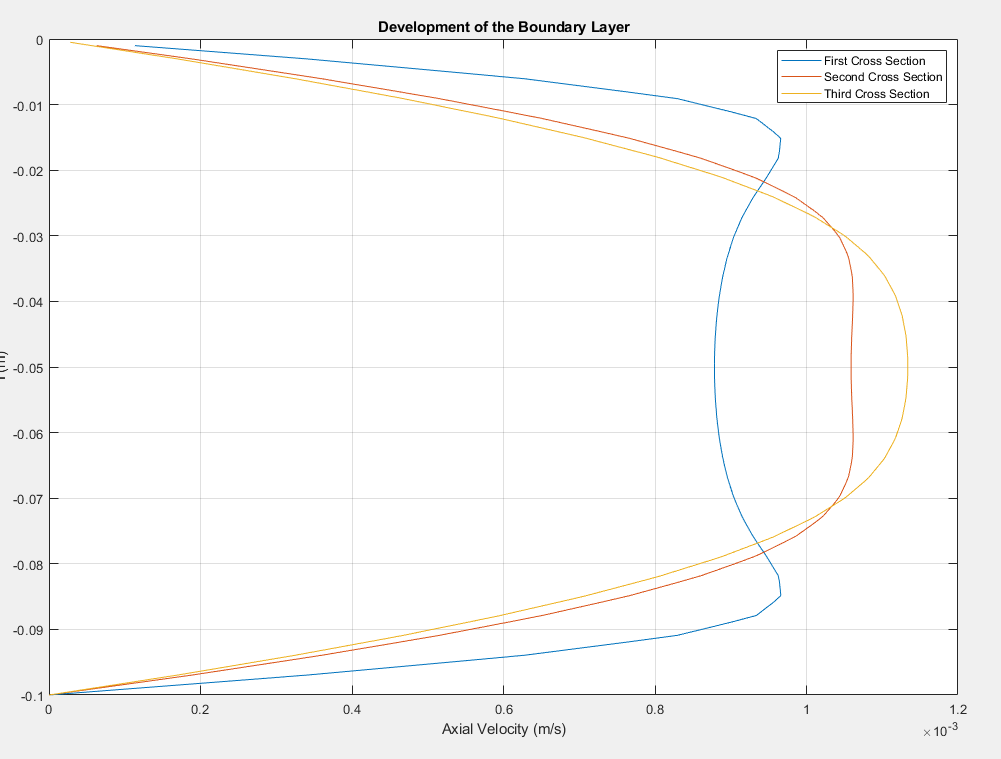
\includegraphics[width=.7\textwidth]{images/task1/development.png}
    \caption{Development of the Boundary Layer}
    \label{fig:development}
\end{figure}

It can be said that the flow develops fully after around the halfway point of the straight line segment. The increased Reynolds number negatively affects the boundary layer. As Re increases, the flow becomes less layered and more unsteady. It can be said that the boundary layer develops earlier for flows with lower Reynolds number. For further information, the pressure contours and streamlines can be found on Figure \ref{fig:press_stream}. 

\begin{figure}[H]
 \centering
\begin{subfigure}{.45\textwidth}
  \centering
  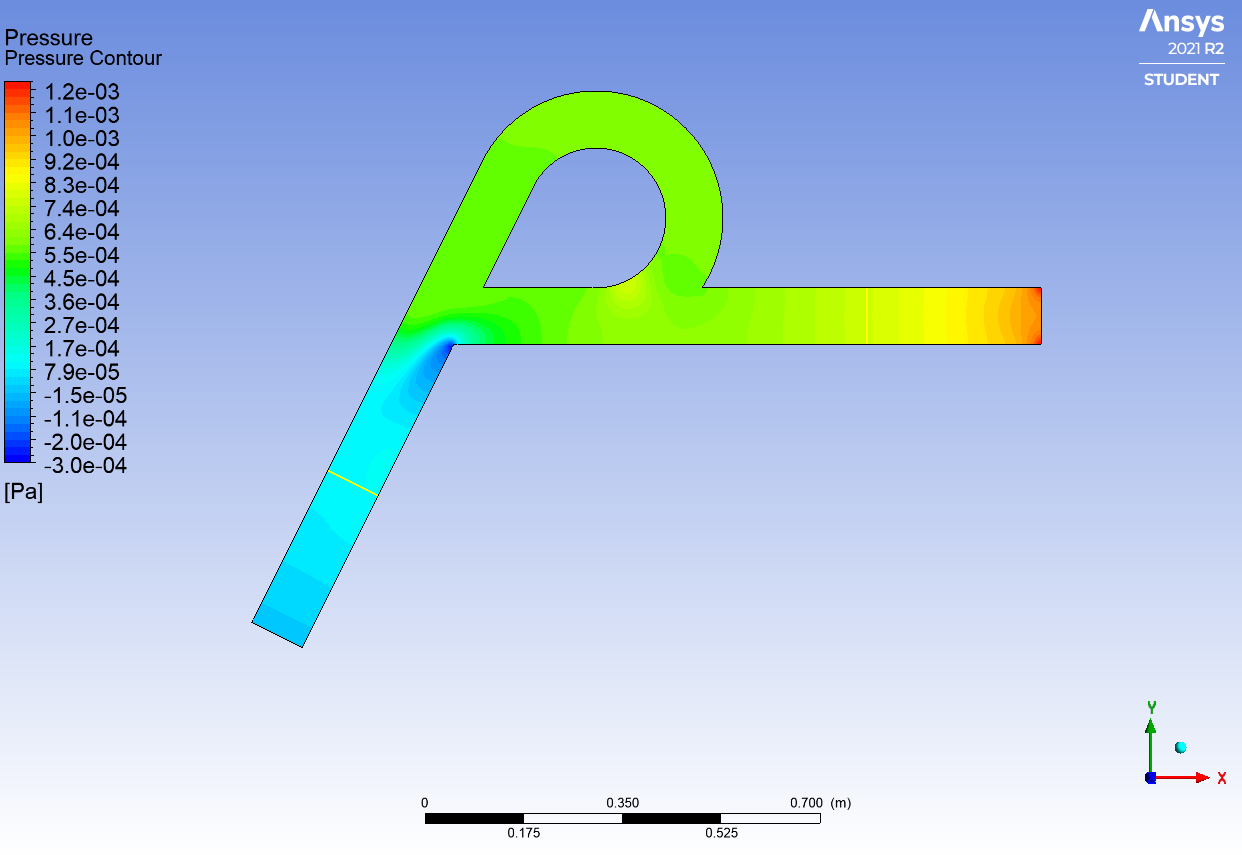
\includegraphics[width=.9\linewidth]{images/task1/6_pressures.png}
  \caption{Pressure Plot for Forward Flow}
  \label{fig:x_d_norm}
\end{subfigure}%
~
\begin{subfigure}{.45\textwidth}
  \centering
  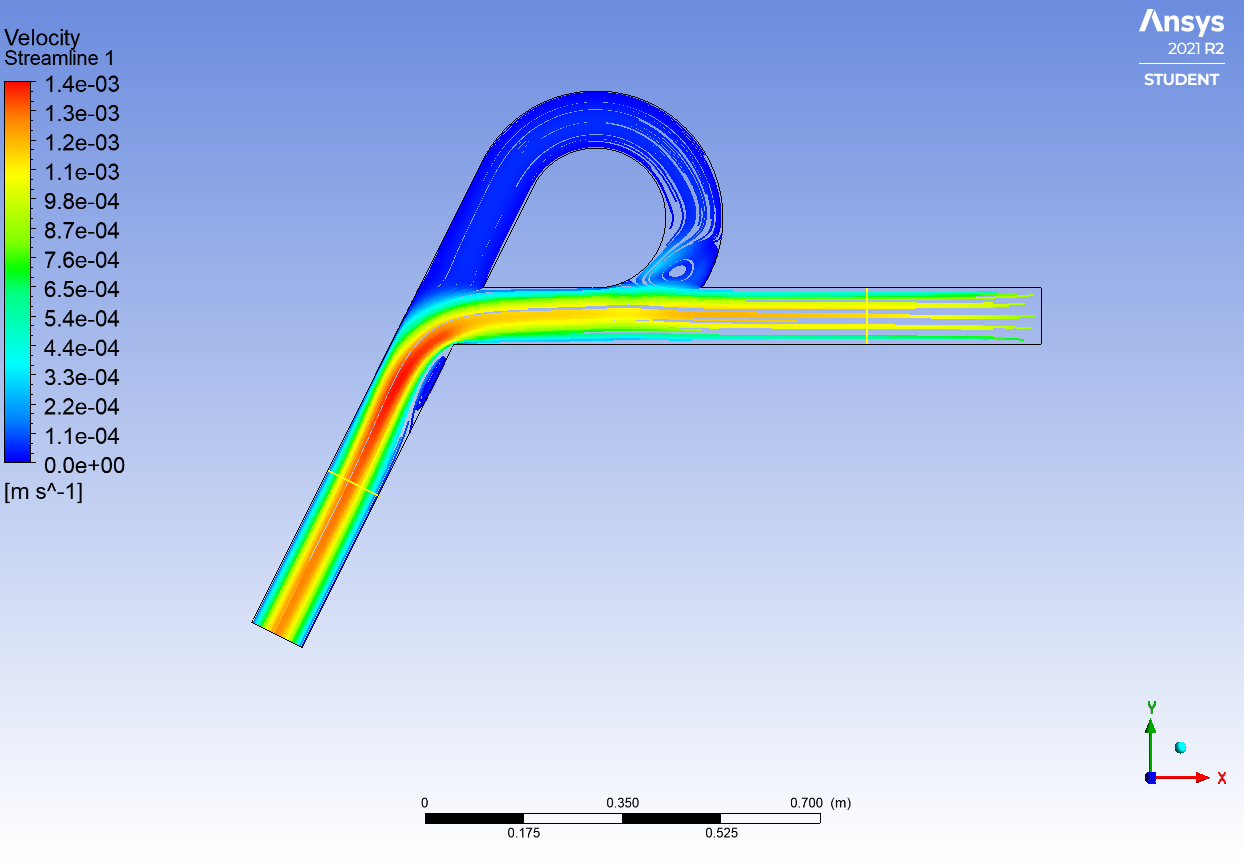
\includegraphics[width=.9\linewidth]{images/task1/6_streamlines.png}
  \caption{Streamlines}
  \label{fig:x_d_norm_actual}
\end{subfigure}
~


\caption{Pressure contours and Streamlines}
\label{fig:press_stream}
\end{figure}
\subsection{Task 2 Results}
\label{sec:task2results}
\subsubsection{Geometry and Mesh}
As far as grid convergence goes, the same setup, mesh size and material properties, along with adapted boundary conditions have been used in this section. As before, it largest element size was no greater than $3x10^{-3}$m. Many different standalone systems were created inside ANSYS Project Schematic by duplicating the geometries and modifying them to agree with the new Reynolds number and different $L$ values. A sample sketch of the valvular conduit with $L=400$mm and $Re=181$ is shown in Figure \ref{fig:examplesketch} below.\\

\begin{figure}[H]
    \centering
    
\includegraphics[width = .8\textwidth]{images/task2/sketch_examples/re181.png}
    \caption{Sketch for Re=181 and L=400mm}
    \label{fig:examplesketch}
\end{figure}

\subsubsection{Diodicity Calculations}
The dimensions of the geometry has been modified in each step in accordance with the corresponding Reynolds Numbers and pressure drops in each step have been calculated which is then plugged in to the diodicity formula. The corresponding diodicities are shown on Table \ref{tab:diodicities} below. These results will then be plotted and a curve will be fitted to extract the optimum values.




\begin{table}[H]
\centering
\caption{Diodicities of all configurations}
\label{tab:diodicities}
\resizebox{.4\textwidth}{!}{%
\begin{tabular}{c|ccc}
\hline
\multirow{2}{*}{Re} & \multicolumn{3}{c}{L (mm)}                                      \\ \cline{2-4} 
                    & \multicolumn{1}{c|}{200}   & \multicolumn{1}{c|}{400}   & 600   \\ \hline
181                 & \multicolumn{1}{c|}{1.295} & \multicolumn{1}{c|}{1.200} & 1.131 \\ \hline
362                 & \multicolumn{1}{c|}{1.635} & \multicolumn{1}{c|}{1.705} & 1.471 \\ \hline
543                 & \multicolumn{1}{c|}{1.813} & \multicolumn{1}{c|}{2.434} & 2.244 \\ \hline
\end{tabular}%
}
\end{table}





As can be seen from Figures \ref{fig:l200}, \ref{fig:l400} and \ref{fig:l600} below, pressure values change significantly between the forward and reverse flow cases. Using these plots and the probe method from ANSYS, the pressure drops were calculated. 


%%%%%%%%%%%%%%% L = 200 %%%%%%%%%%%%%
\begin{figure}[H]
 \centering
\begin{subfigure}{.45\textwidth}
  \centering
  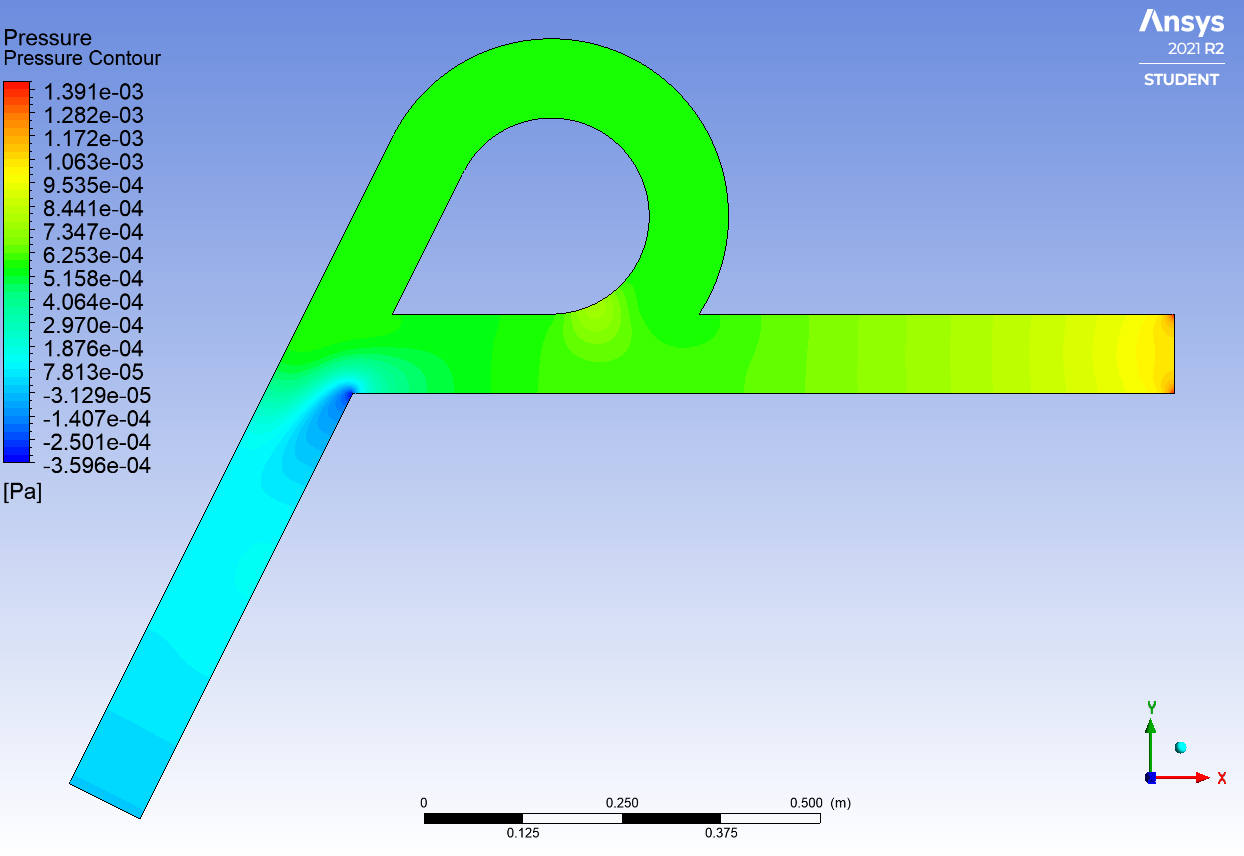
\includegraphics[width=.9\linewidth]{images/task2/L200/forward181.png}
  \caption{Forward flow Re = 181}
  \label{fig:x_d_norm}
\end{subfigure}%
~
\begin{subfigure}{.45\textwidth}
  \centering
  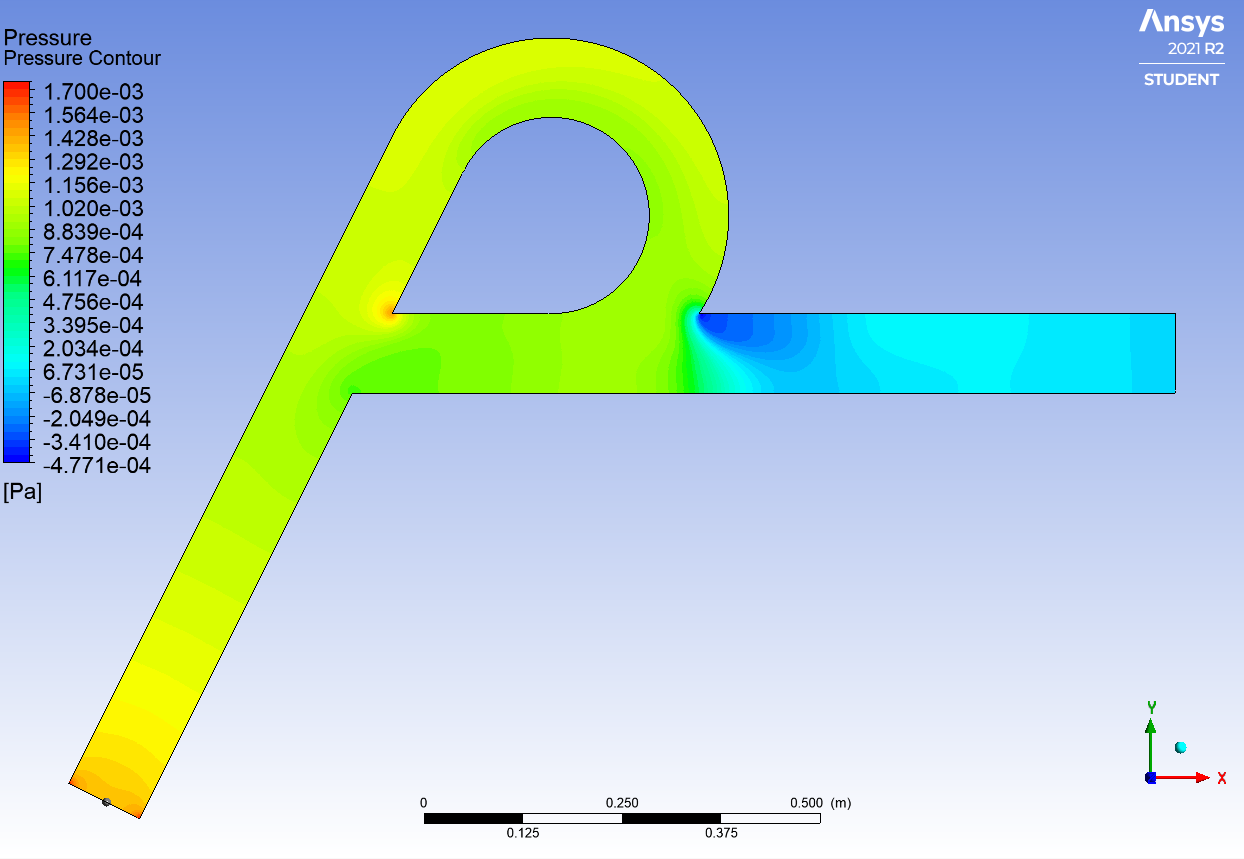
\includegraphics[width=.9\linewidth]{images/task2/L200/reverse181.png}
  \caption{Reverse flow with Re = 181}
  \label{fig:x_d_norm_actual}
\end{subfigure}
~
\begin{subfigure}{.45\textwidth}
  \centering
  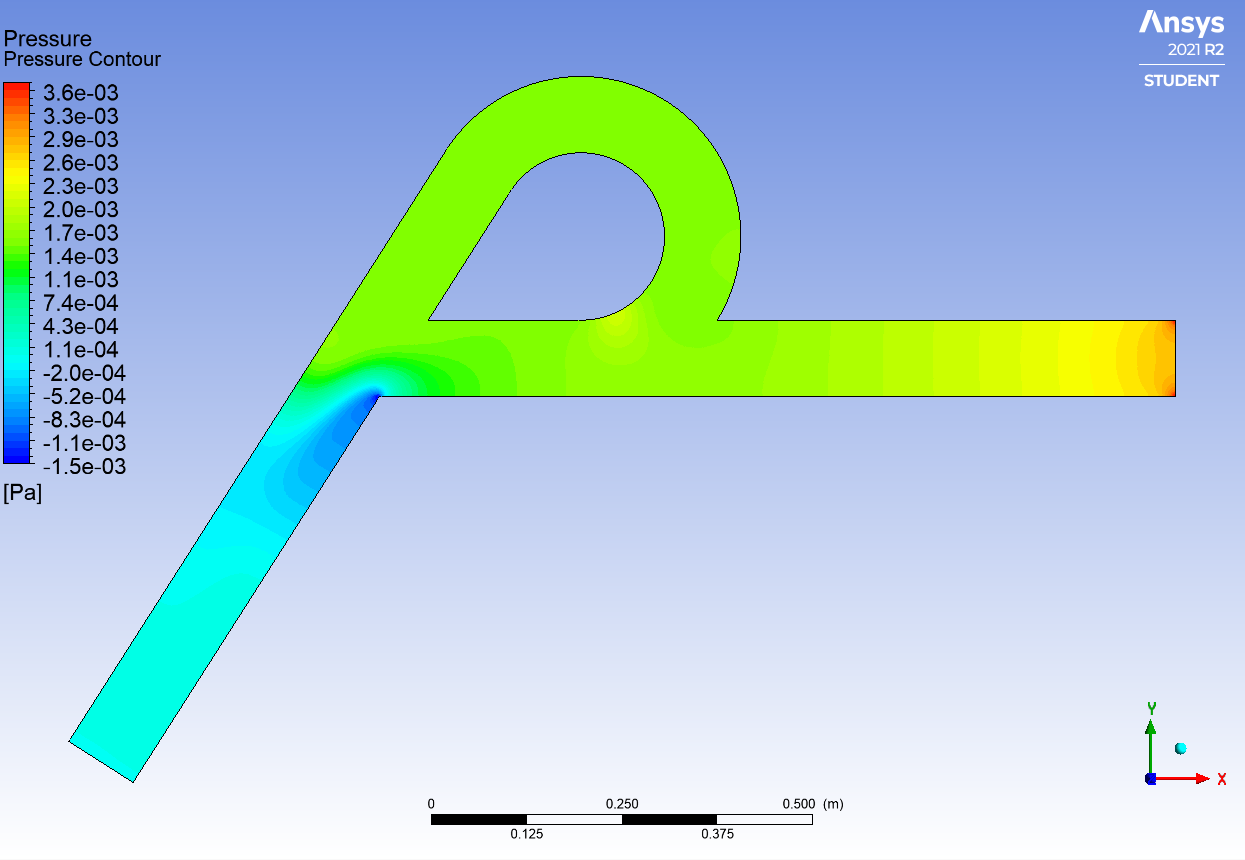
\includegraphics[width=.9\linewidth]{images/task2/L200/forward362.png}
  \caption{Forward flow Re = 362}
  \label{fig:x_d_norm}
\end{subfigure}%
~
\begin{subfigure}{.45\textwidth}
  \centering
  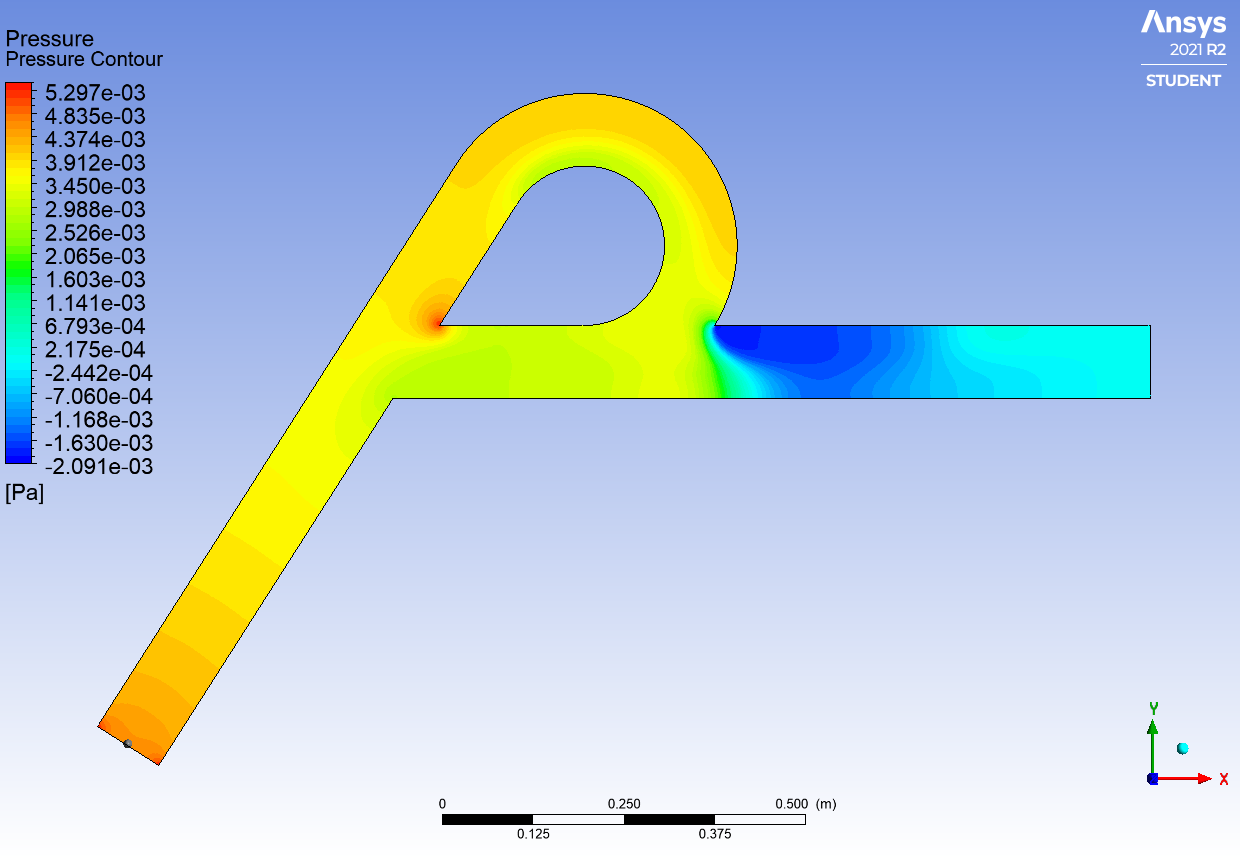
\includegraphics[width=.9\linewidth]{images/task2/L200/reverse362.png}
  \caption{Reverse flow with Re = 362}
  \label{fig:x_d_norm_actual}
\end{subfigure}
~
\begin{subfigure}{.45\textwidth}
  \centering
  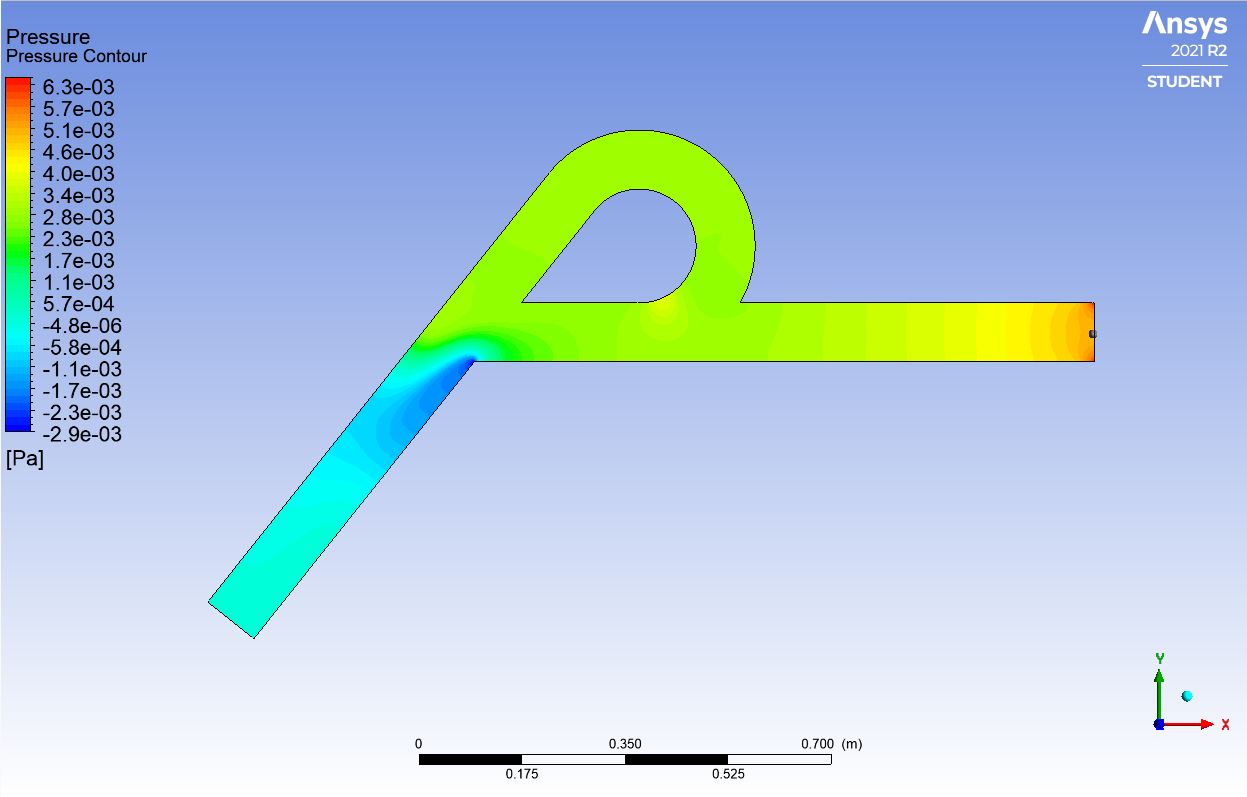
\includegraphics[width=.9\linewidth]{images/task2/L200/forward543.png}
  \caption{Forward flow Re = 543}
  \label{fig:x_d_norm}
\end{subfigure}%
~
\begin{subfigure}{.45\textwidth}
  \centering
  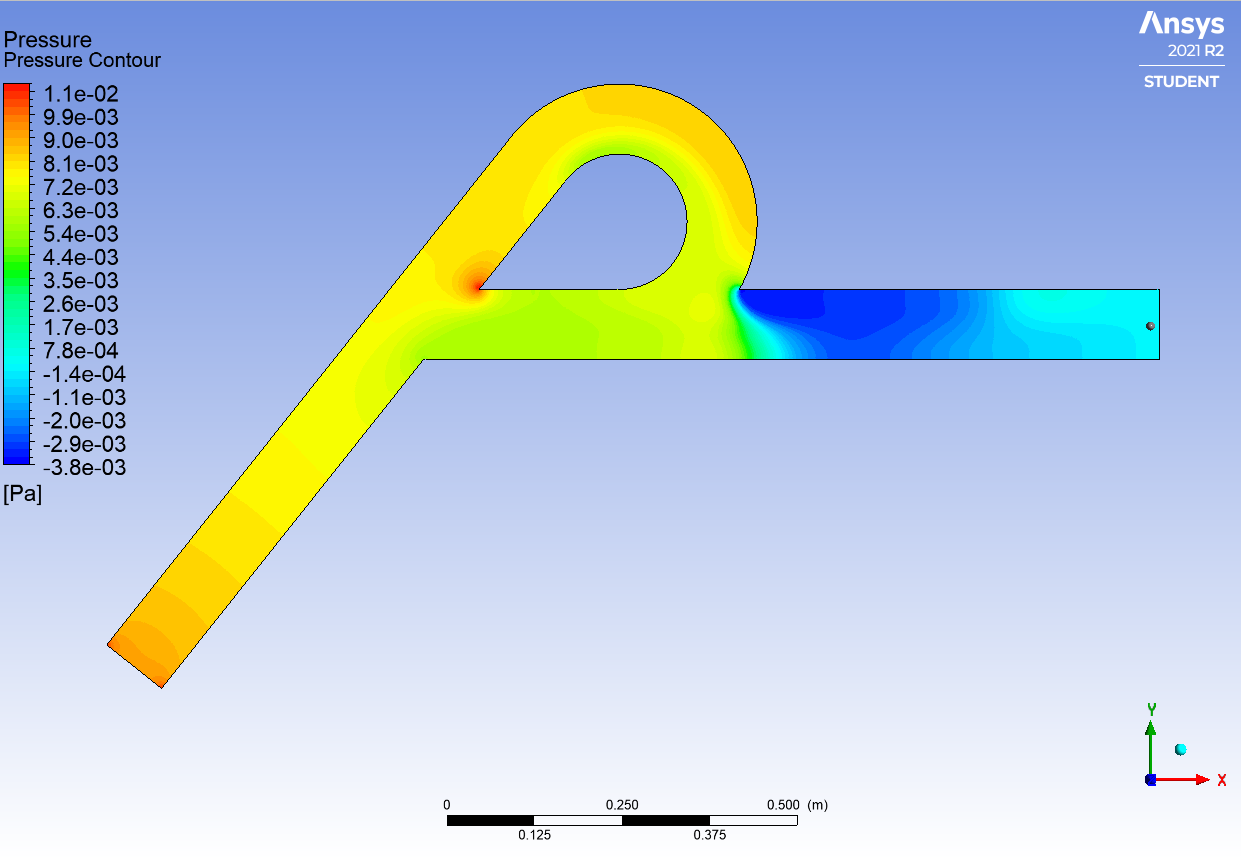
\includegraphics[width=.9\linewidth]{images/task2/L200/reverse543.png}
  \caption{Reverse flow with Re = 543}
  \label{fig:x_d_norm_actual}
\end{subfigure}

\caption{Different Pressure Plots where L = 200mm}
\label{fig:l200}
\end{figure}





%%%%%%%%%% L = 400 %%%%%%%%%%%%%%%%
\begin{figure}[H]
 \centering
\begin{subfigure}{.45\textwidth}
  \centering
  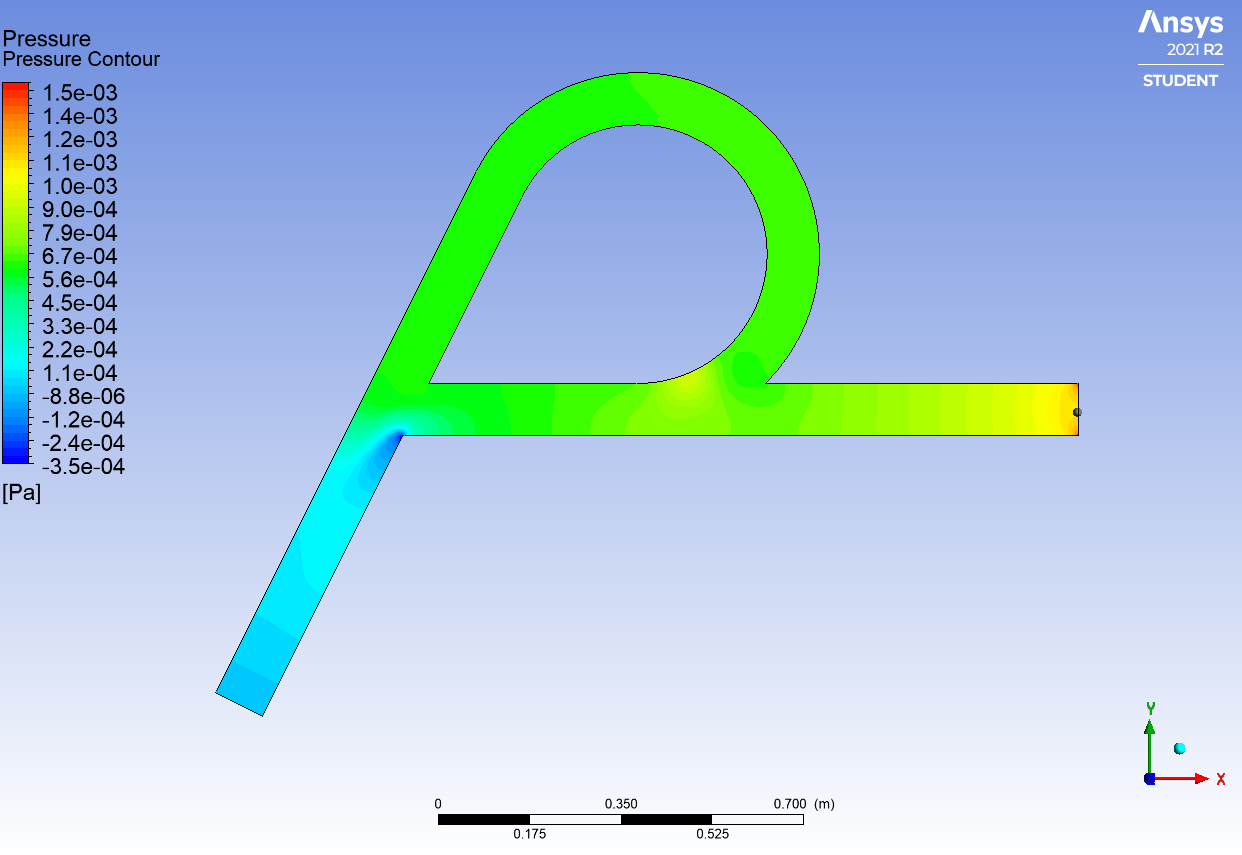
\includegraphics[width=.9\linewidth]{images/task2/L400/forward181.png}
  \caption{Forward flow Re = 181}
  \label{fig:x_d_norm}
\end{subfigure}%
~
\begin{subfigure}{.45\textwidth}
  \centering
  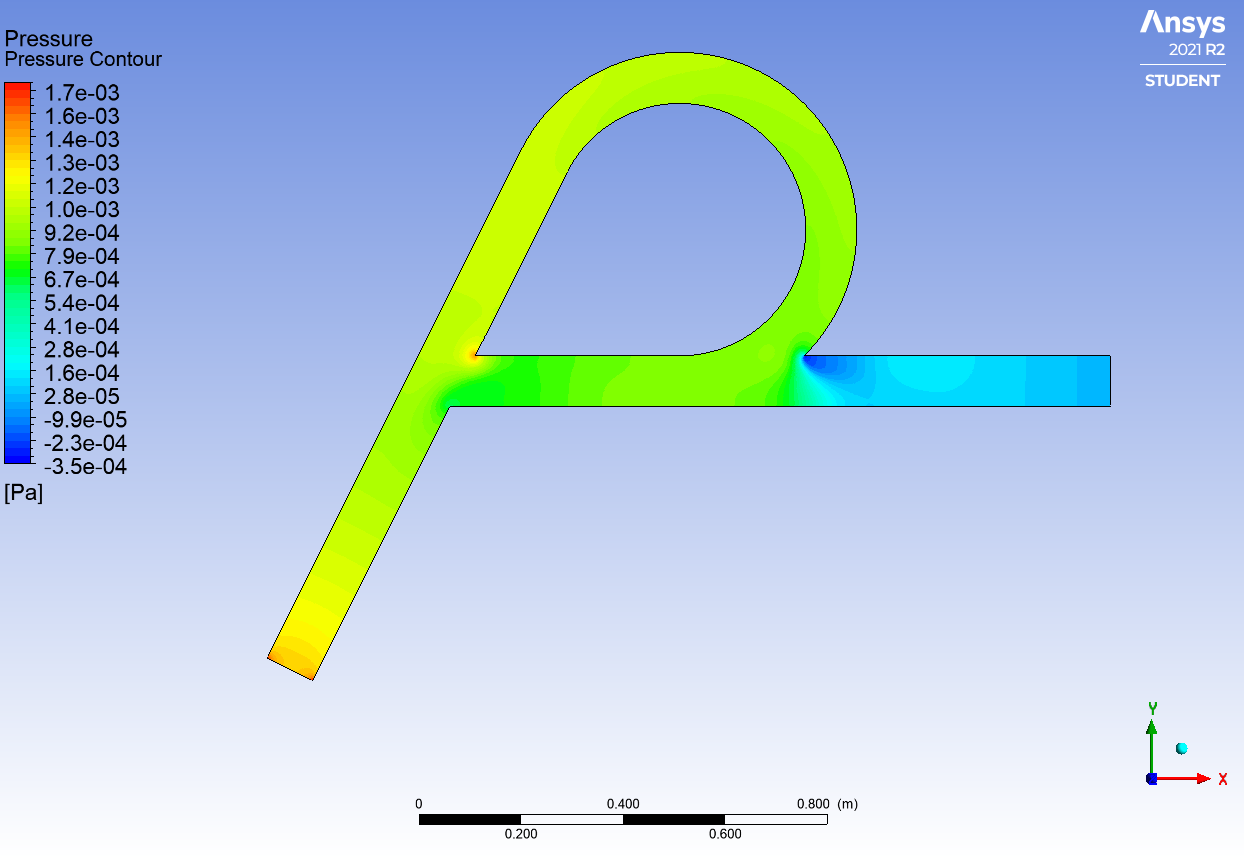
\includegraphics[width=.9\linewidth]{images/task2/L400/reverse181.png}
  \caption{Reverse flow with Re = 181}
  \label{fig:x_d_norm_actual}
\end{subfigure}
~
\begin{subfigure}{.45\textwidth}
  \centering
  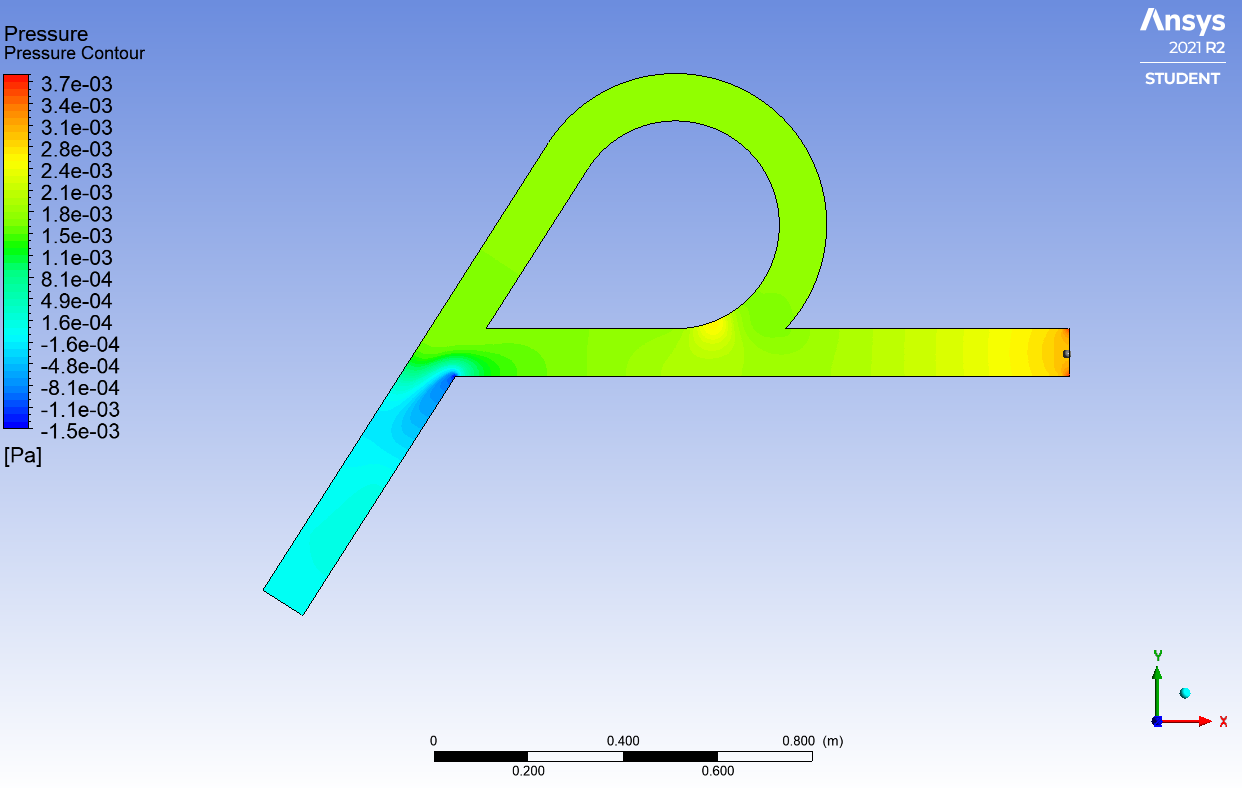
\includegraphics[width=.9\linewidth]{images/task2/L400/forward362.png}
  \caption{Forward flow Re = 362}
  \label{fig:x_d_norm}
\end{subfigure}%
~
\begin{subfigure}{.45\textwidth}
  \centering
  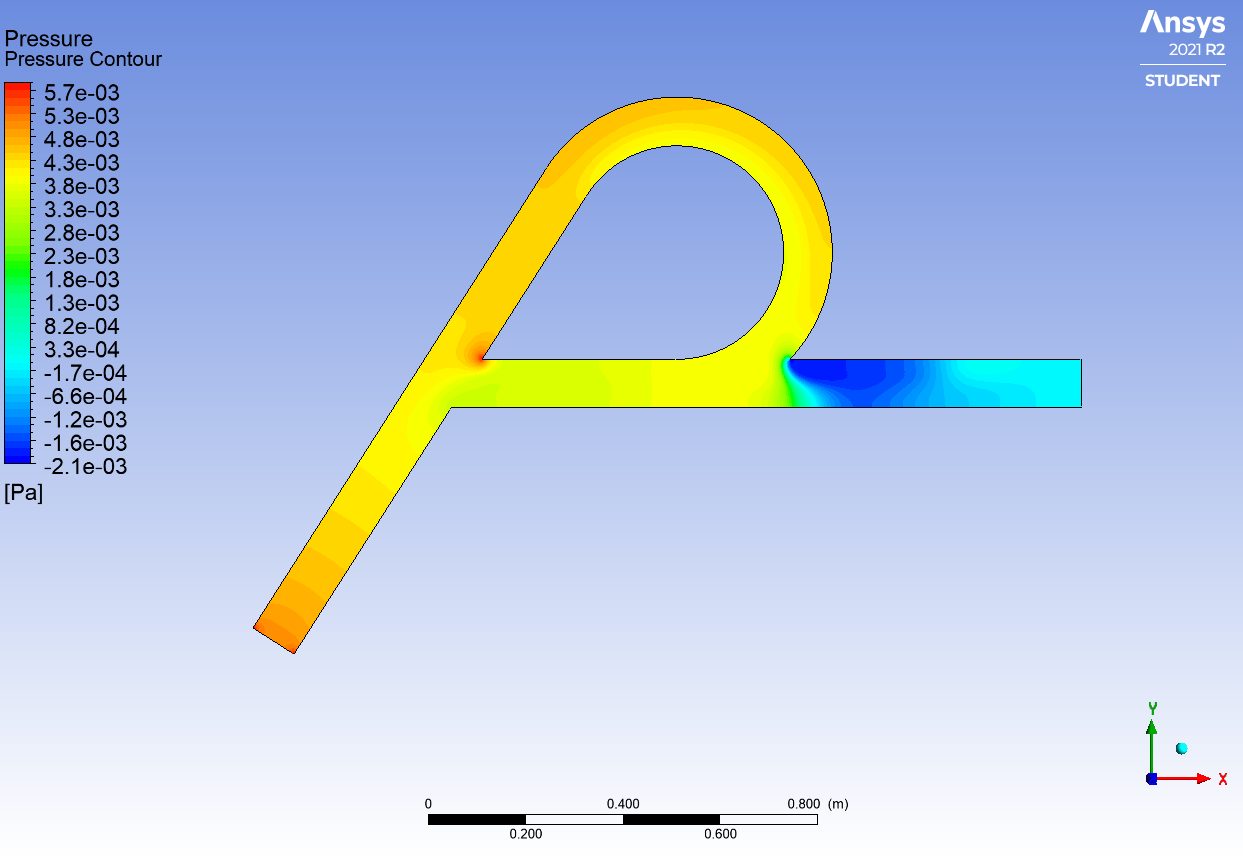
\includegraphics[width=.9\linewidth]{images/task2/L400/reverse362.png}
  \caption{Reverse flow with Re = 362}
  \label{fig:x_d_norm_actual}
\end{subfigure}
~
\begin{subfigure}{.45\textwidth}
  \centering
  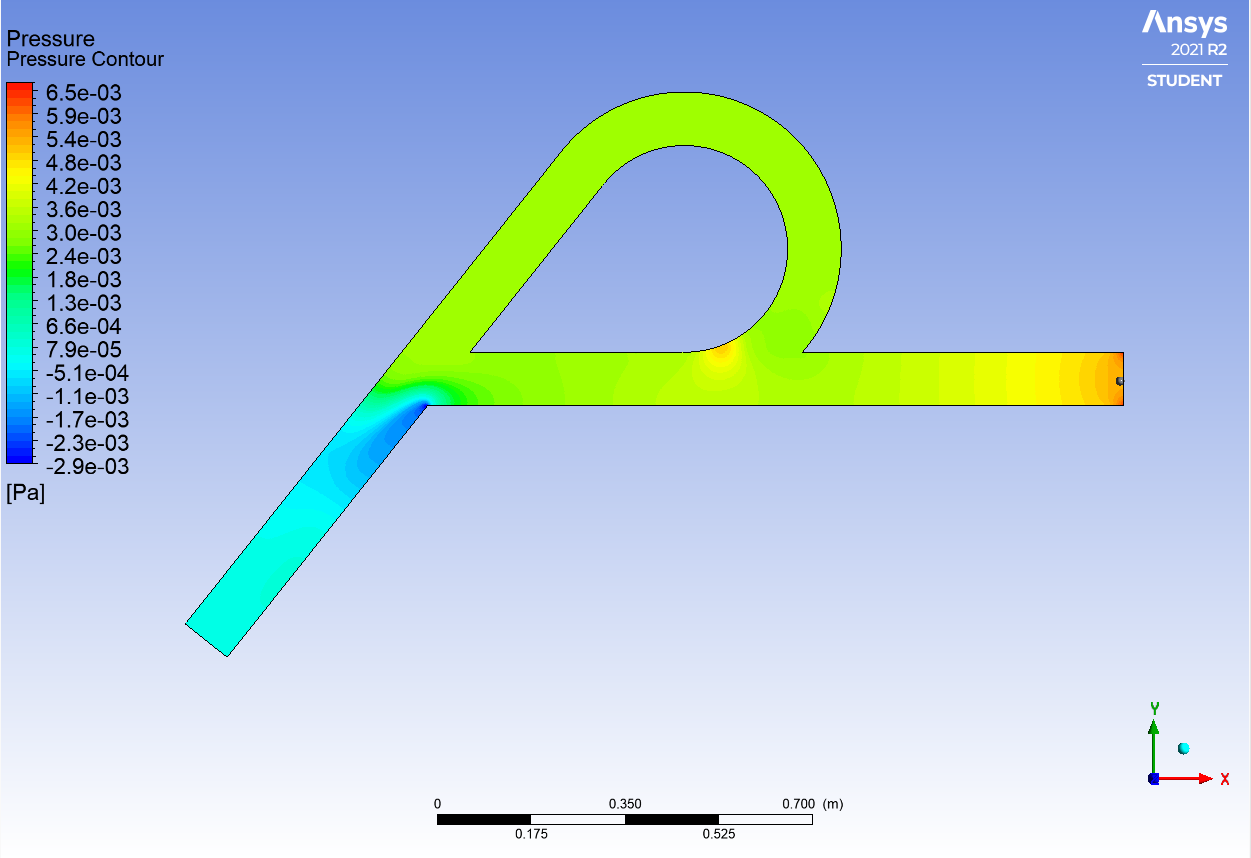
\includegraphics[width=.9\linewidth]{images/task2/L400/forward543.png}
  \caption{Forward flow Re = 543}
  \label{fig:x_d_norm}
\end{subfigure}%
~
\begin{subfigure}{.45\textwidth}
  \centering
  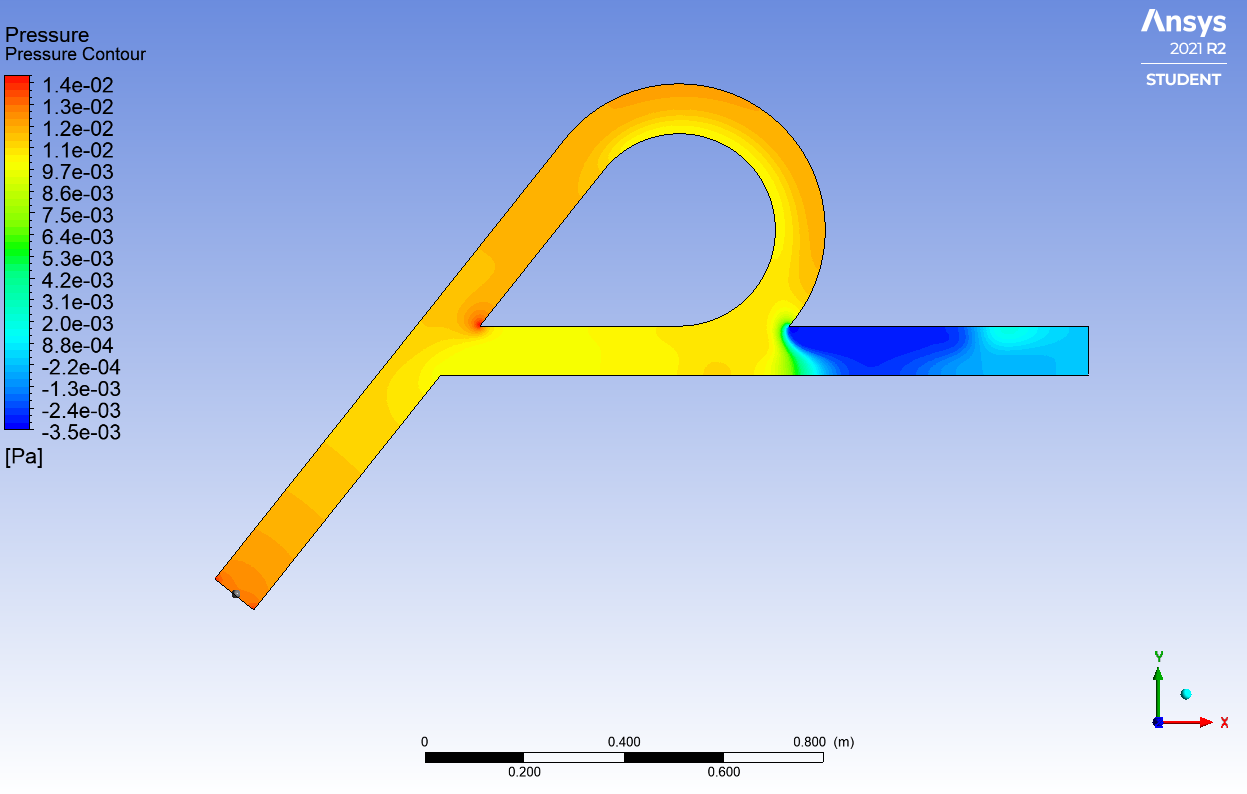
\includegraphics[width=.9\linewidth]{images/task2/L400/reverse543.png}
  \caption{Reverse flow with Re = 543}
  \label{fig:x_d_norm_actual}
\end{subfigure}

\caption{Different Pressure Plots where L = 400mm}
\label{fig:l400}
\end{figure}


%%%%%%%%%% L = 600 %%%%%%%%%%%%%%%%
\begin{figure}[H]
 \centering
\begin{subfigure}{.45\textwidth}
  \centering
  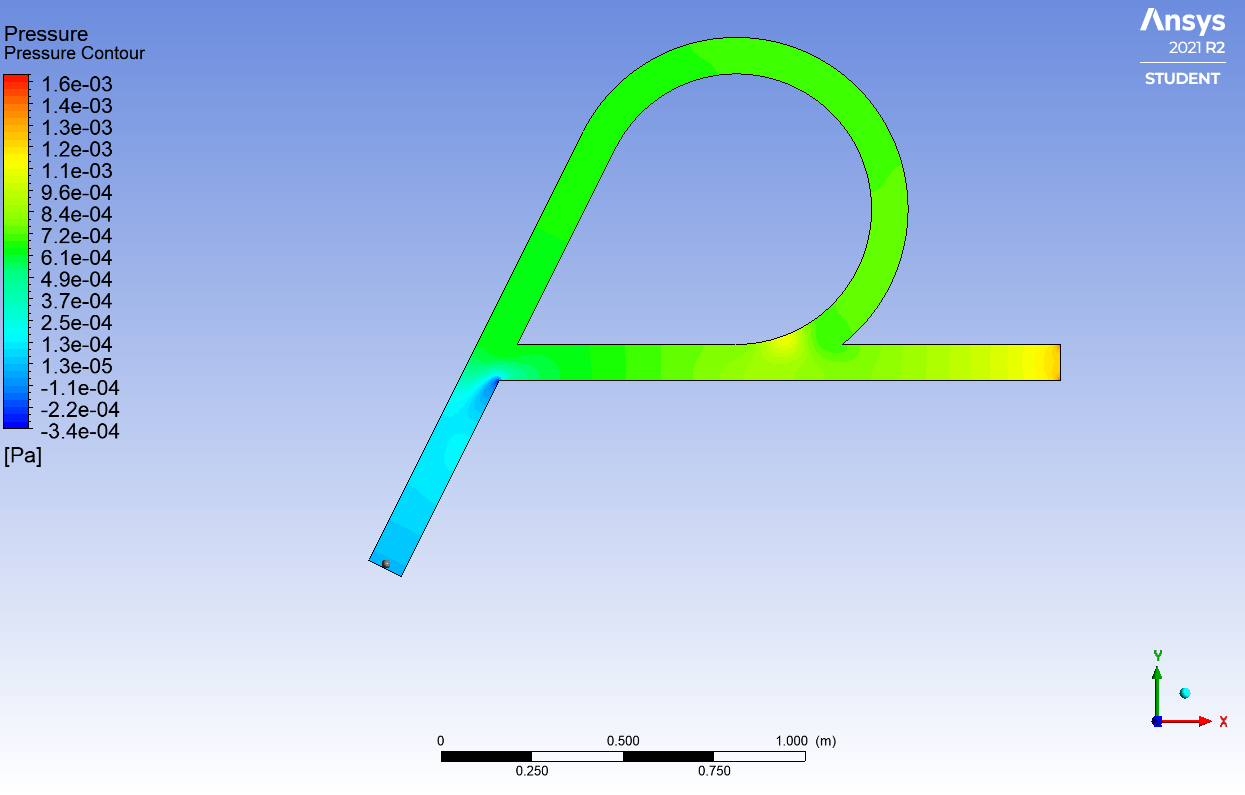
\includegraphics[width=.9\linewidth]{images/task2/L600/forward181.png}
  \caption{Forward flow Re = 181}
  \label{fig:x_d_norm}
\end{subfigure}%
~
\begin{subfigure}{.45\textwidth}
  \centering
  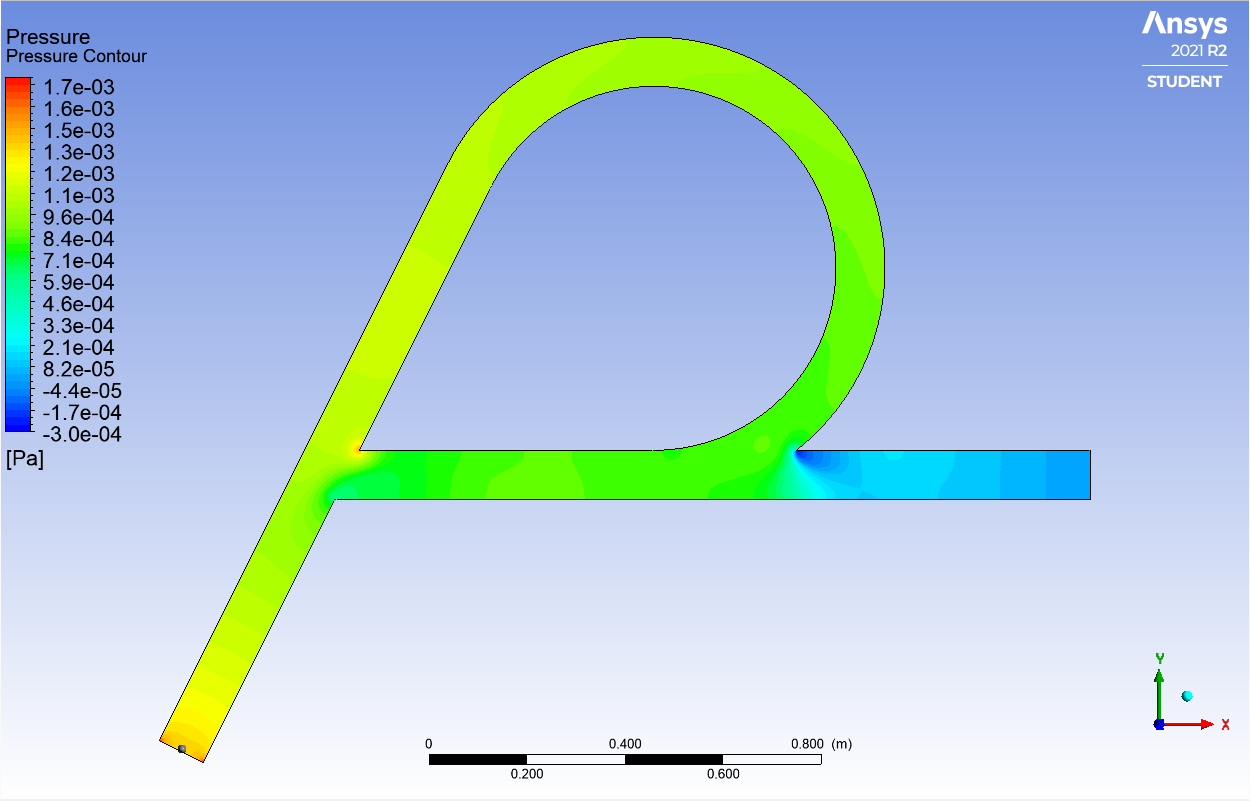
\includegraphics[width=.9\linewidth]{images/task2/L600/reverse181.png}
  \caption{Reverse flow with Re = 181}
  \label{fig:x_d_norm_actual}
\end{subfigure}
~
\begin{subfigure}{.45\textwidth}
  \centering
  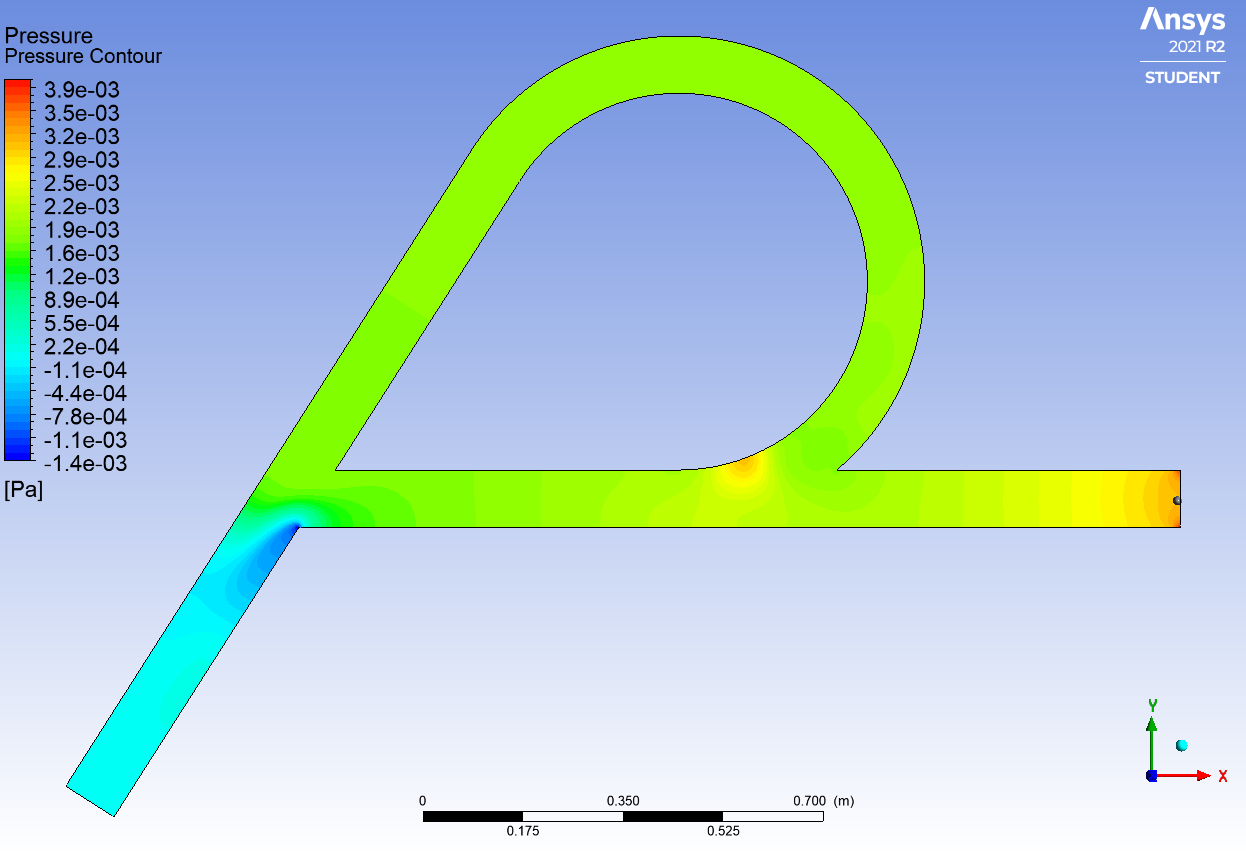
\includegraphics[width=.9\linewidth]{images/task2/L600/forward362.png}
  \caption{Forward flow Re = 362}
  \label{fig:x_d_norm}
\end{subfigure}%
~
\begin{subfigure}{.45\textwidth}
  \centering
  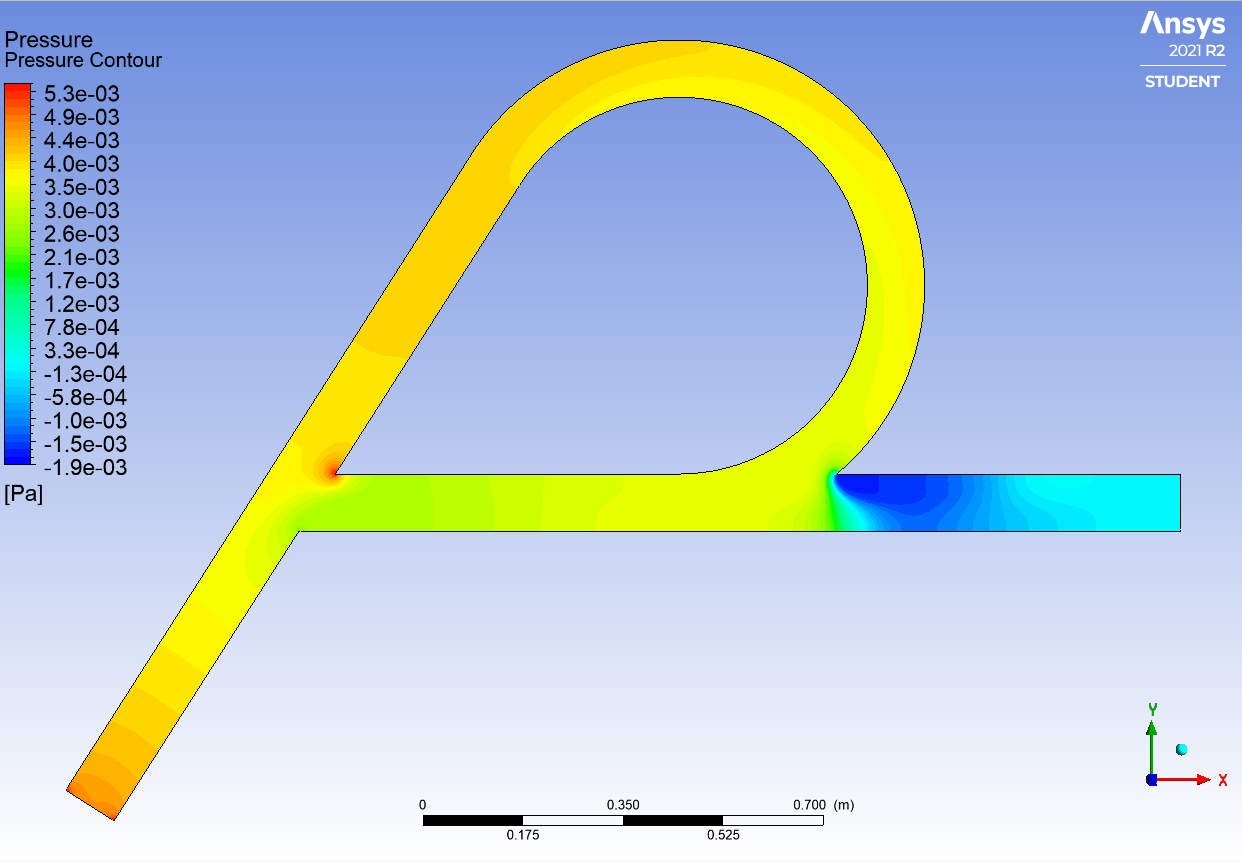
\includegraphics[width=.9\linewidth]{images/task2/L600/reverse362.png}
  \caption{Reverse flow with Re = 362}
  \label{fig:x_d_norm_actual}
\end{subfigure}
~
\begin{subfigure}{.45\textwidth}
  \centering
  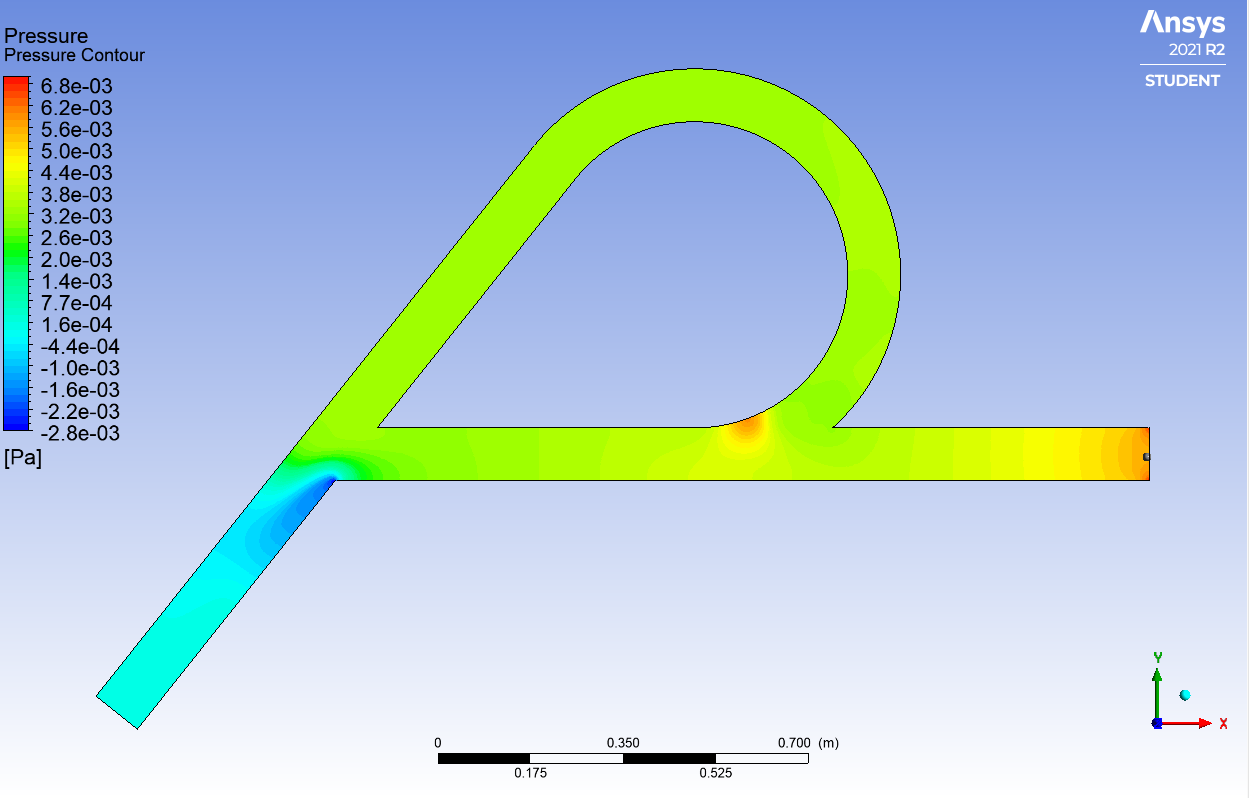
\includegraphics[width=.9\linewidth]{images/task2/L600/forward543.png}
  \caption{Forward flow Re = 543}
  \label{fig:x_d_norm}
\end{subfigure}%
~
\begin{subfigure}{.45\textwidth}
  \centering
  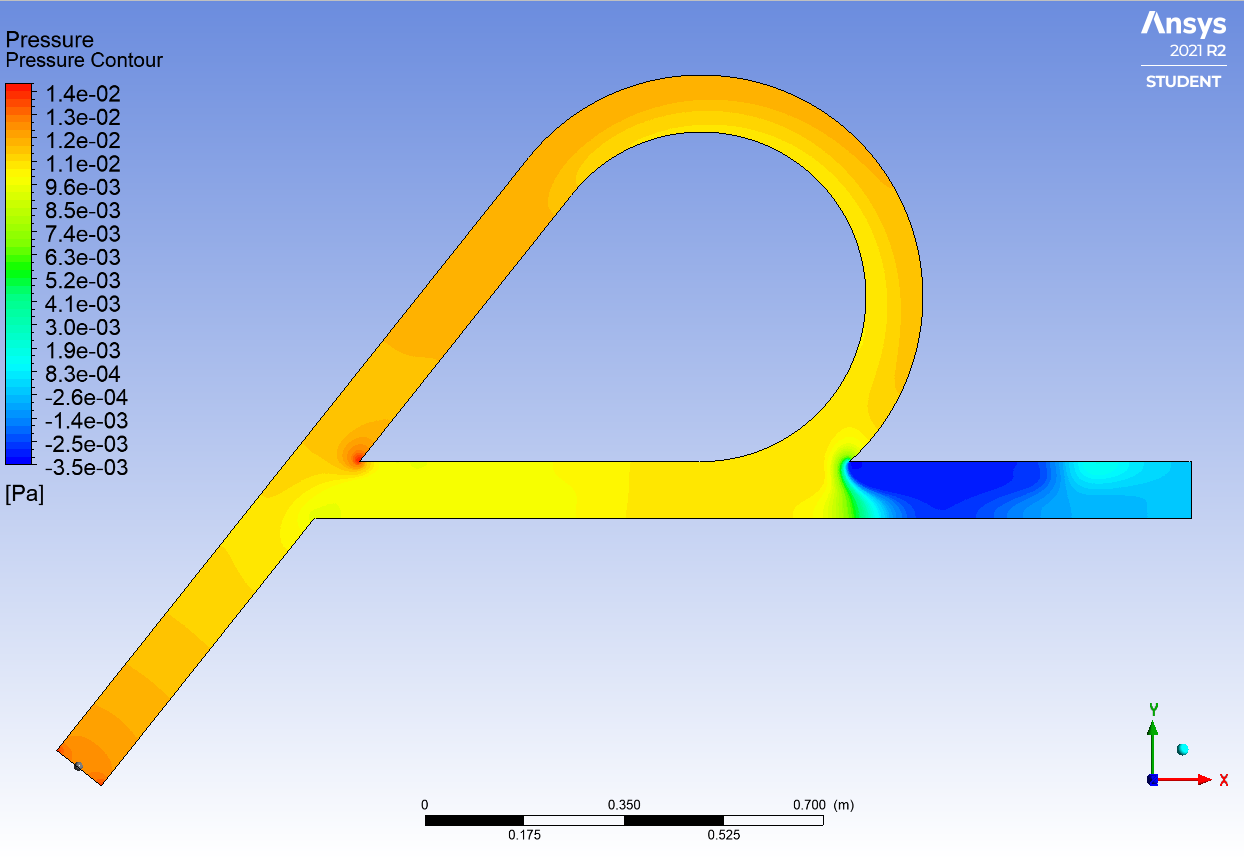
\includegraphics[width=.9\linewidth]{images/task2/L600/reverse543.png}
  \caption{Reverse flow with Re = 543}
  \label{fig:x_d_norm_actual}
\end{subfigure}

\caption{Different Pressure Plots where L = 600mm}
\label{fig:l600}
\end{figure}

\subsubsection{Optimization}

Following these steps, valvular conduit diodicities are plotted versus the straight line segments for all 3 of tested Reynolds numbers. After this, polynomial curves have been fitted to the data in order to find the optimum $L$ values which will be used to relate the optimum $L$ values to Reynolds number. The said plot can be seen on Figure \ref{fig:diodi_vs_L} along with their corresponding fitted polynomial curves. The optimum L values extracted for all 3 Reynolds numbers are found as follows:
\begin{itemize}
    \item Re = 181 : $L_{opt} = 450$
    \item Re = 362 : $L_{opt} = 325$
    \item Re = 543 : $L_{opt} = 200$
\end{itemize}

\begin{figure}[H]
    \centering
    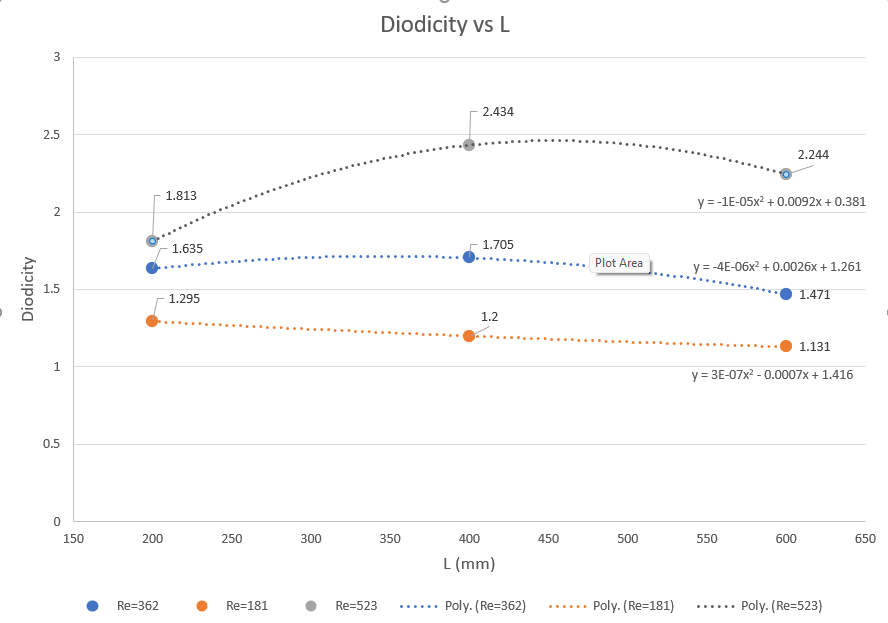
\includegraphics[width = .96\textwidth]{images/task2/diodicity_vs_L_fits.png}
    \caption{Diodicities vs $L$ with plotted curve fits.}
    \label{fig:diodi_vs_L}
\end{figure}


Now that we have the $L_{opt} values$ for 3 different Reynolds numbers, the next step is to try and relate these two and fit a curve accordingly. Figure \ref{fig:LWvsRe} shows this relation along with the equation for the fitted curve. 


\begin{figure}[H]
    \centering
    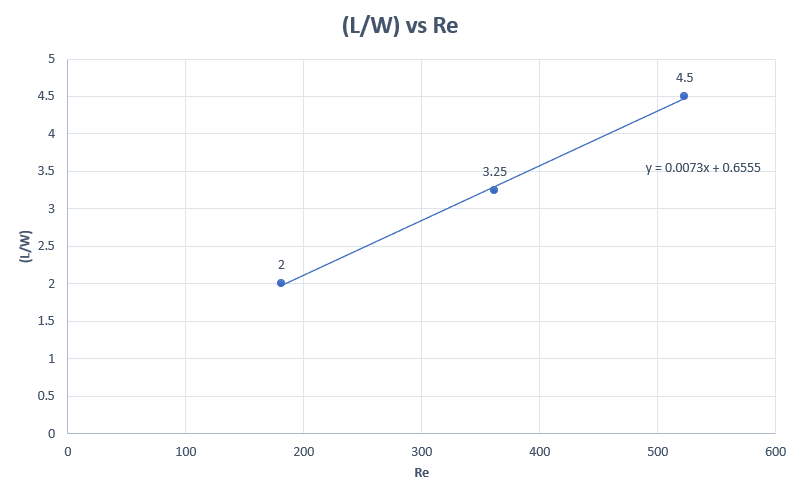
\includegraphics[width = .96\textwidth]{images/task2/LW_vs_Re.png}
    \caption{$(L/W)_{opt} vs Re$}
    \label{fig:LWvsRe}
\end{figure}


It can be clearly seen that the data has shown a linear trend with Reynolds number, the necessary ratio getting greater as Re increases. The fitted relation is as follows:

\begin{equation}
    (L/W)_{opt} = 0.65 + 0.007 * Re
\end{equation}

When compared with Truong's solution \cite{truong}, it can be clearly seen that the equations agree, having the same slope and very little error in constant value. For comparison Truong's solution is found as below:
\begin{equation}
    (L/W)_{opt} = 0.58 + 0.007 * Re
\end{equation}


Following these steps, to observe more about this optimization, a new simulation is conducted using Re = 724 and all the optimal parameters available, including the optimized $L$ value found using our own fitted curve. For Re = 724, $L$ is found to be 571.8mm and $\alpha_{opt}$ is found to be $45.408^\circ$. The pressure plots and velocity plots for both directions are shown on Figure \ref{fig:opt}. This configuration resulted in a \textbf{diodicity of 2.89 which is the maximum diodicity found yet.} \\

Besides this maximum diodicity, the pressure plots and velocities are to be discussed. As can be seen clearly, in forward flow, the velocity of the fluid inside the curved section is very low, almost a stable configuration. This allows the curve to interfere significantly less than otherwise. Mainly due to this, we see the less pressure dropped flow in that direction. However, when we examine the same geometry's reverse flow, we see a quite different situation. The fluid is very fast in that section with when united with the straight flow, causes disturbances and results in a very high pressure drop. \\

%%%%%%%%%opt figure %%%%%%%%%%%%%%
\begin{figure}[H]
 \centering
\begin{subfigure}{.45\textwidth}
  \centering
  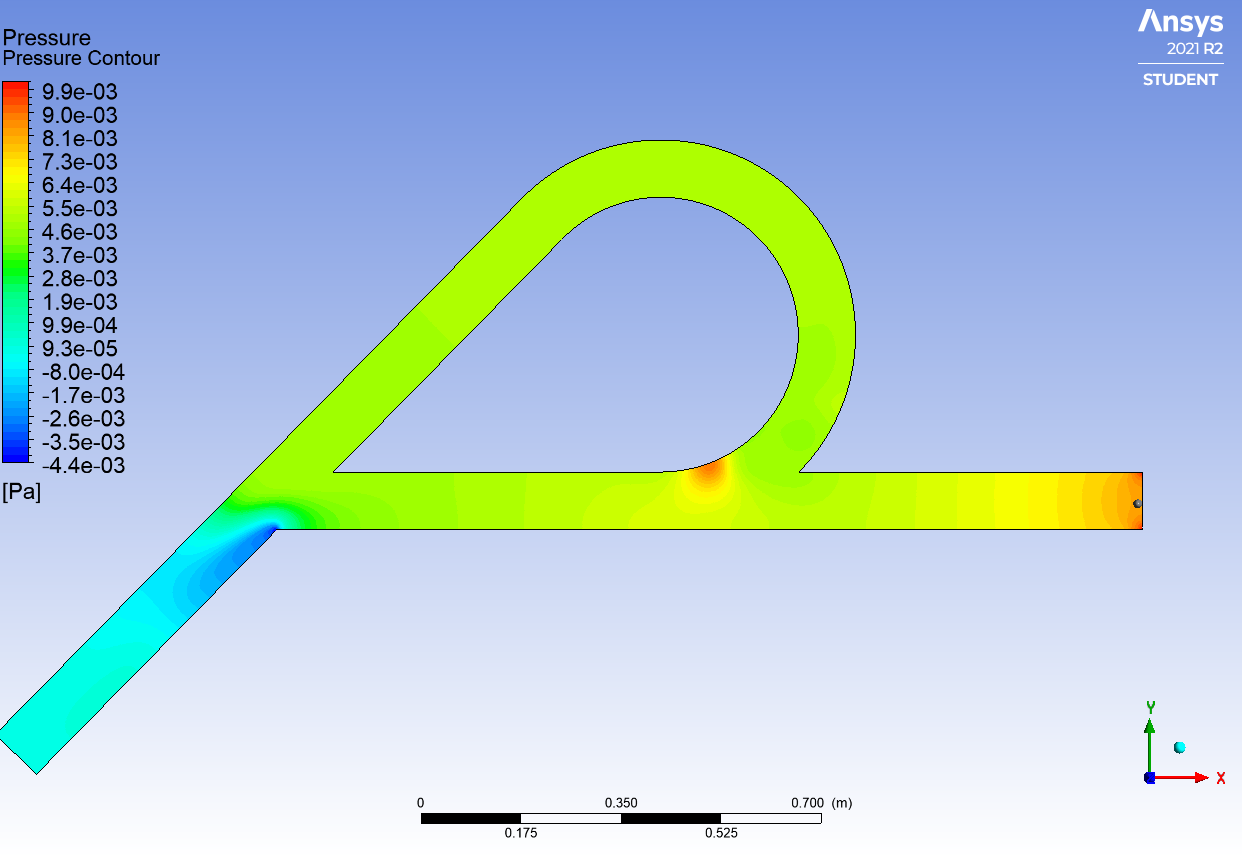
\includegraphics[width=.9\linewidth]{images/task2/myopt/forward_pressure.png}
  \caption{Pressure Plot for Forward Flow}
  \label{fig:x_d_norm}
\end{subfigure}%
~
\begin{subfigure}{.45\textwidth}
  \centering
  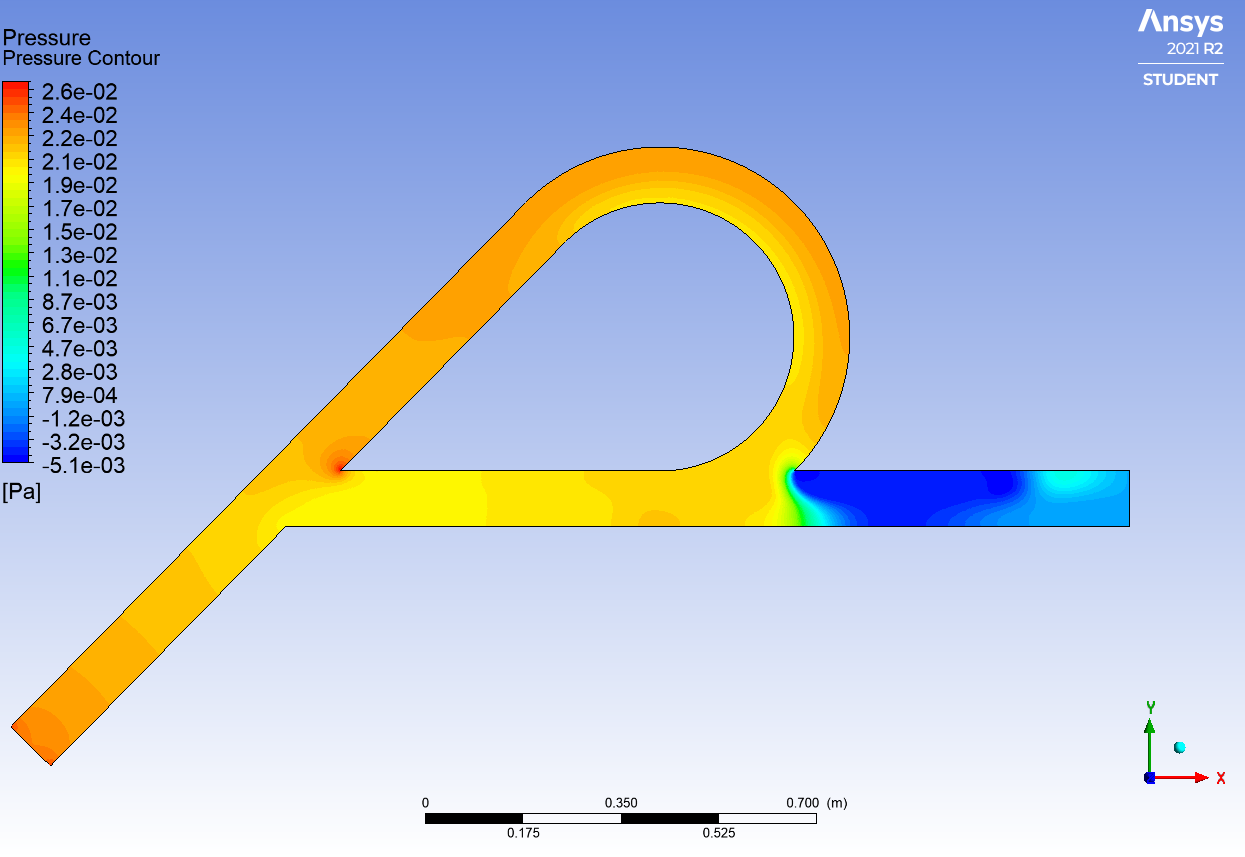
\includegraphics[width=.9\linewidth]{images/task2/myopt/reverse_pressure.png}
  \caption{Pressure Plot for Reverse Flow}
  \label{fig:x_d_norm_actual}
\end{subfigure}
~
\begin{subfigure}{.45\textwidth}
  \centering
  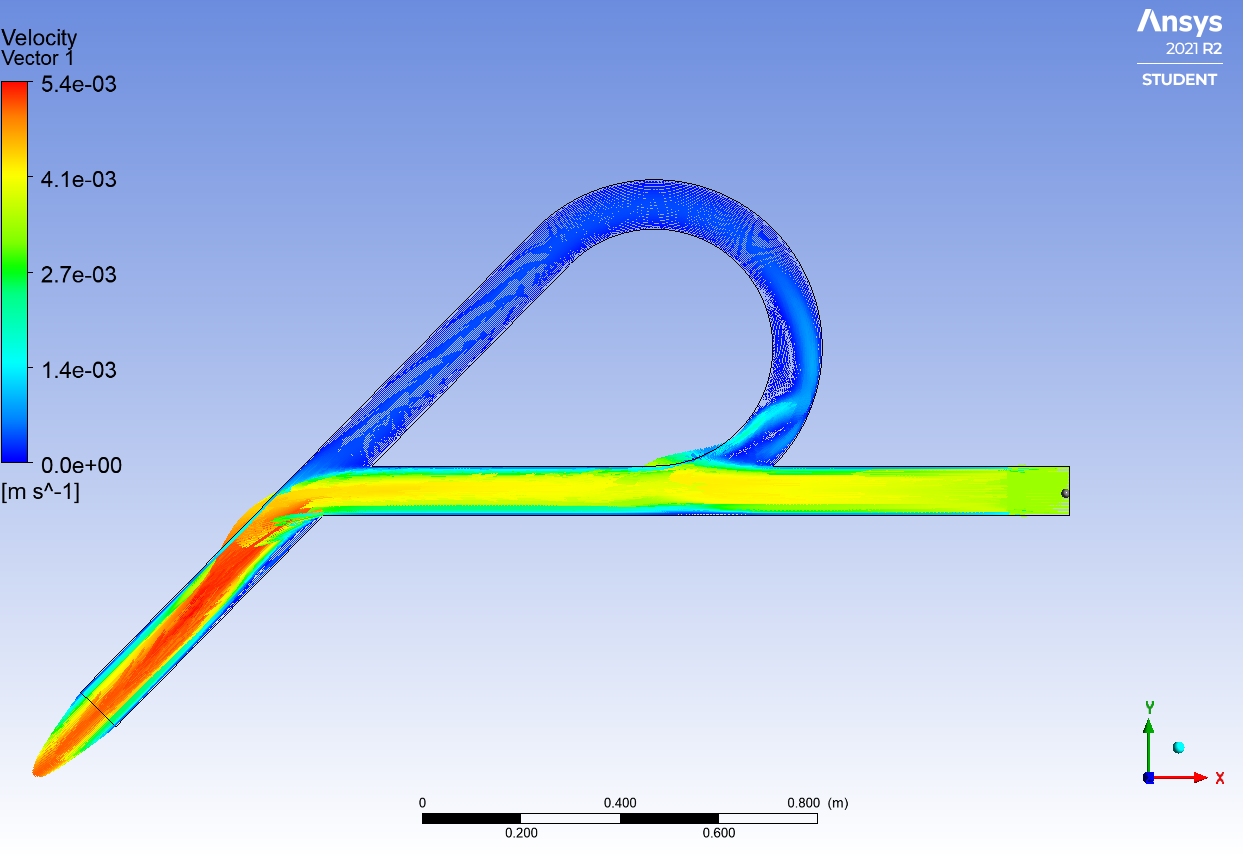
\includegraphics[width=.9\linewidth]{images/task2/myopt/forward_velocity.png}
  \caption{Velocity Plot for Forward Flow}
  \label{fig:x_d_norm}
\end{subfigure}%
~
\begin{subfigure}{.45\textwidth}
  \centering
  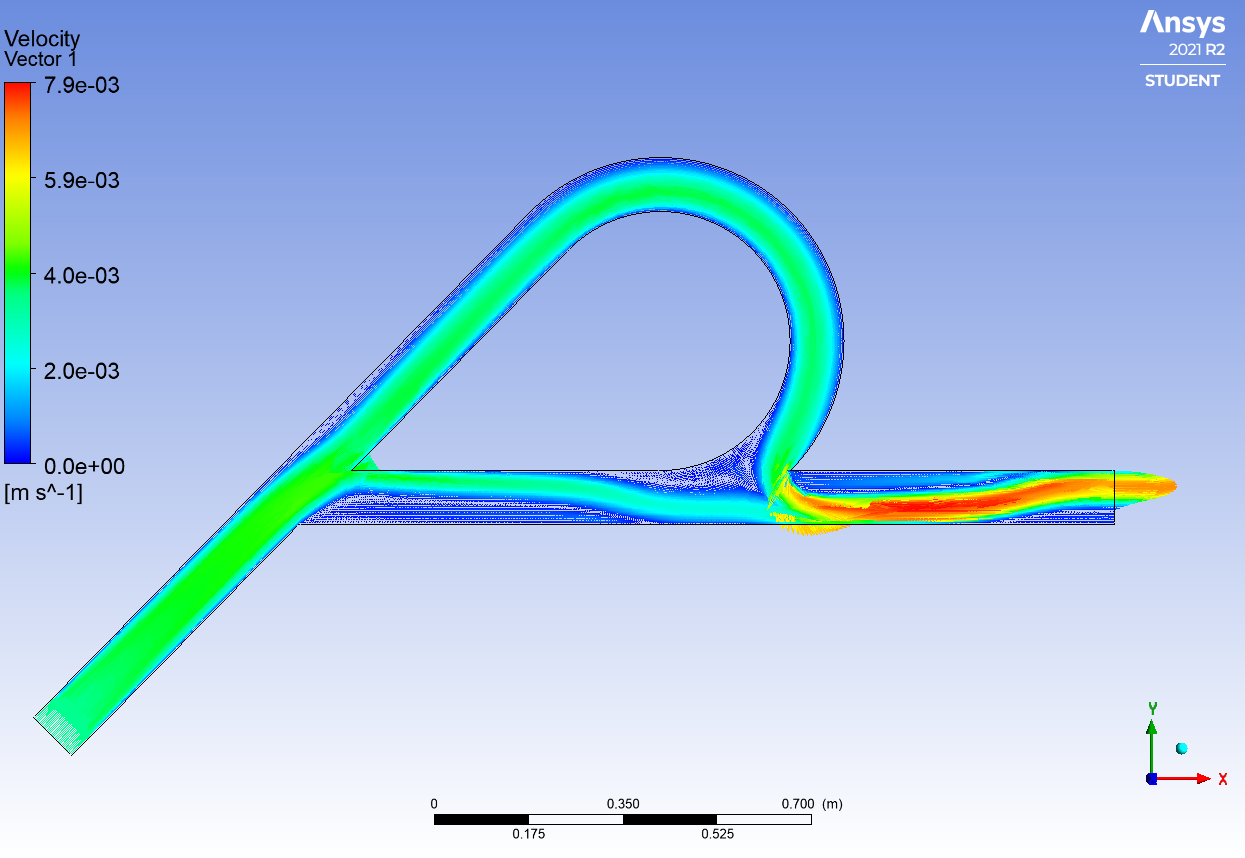
\includegraphics[width=.9\linewidth]{images/task2/myopt/reverse_velocity.png}
  \caption{Velocity Plot for Reverse Flow}
  \label{fig:x_d_norm_actual}
\end{subfigure}

\caption{Optimal L Cases for Re = 724}
\label{fig:opt}
\end{figure}

These comments can also be supported by examining the pressure plots. The pressure plot for reverse flow shows that when high pressured 2 flows are collided at the beginning of the $L_2$ segment, the remaining pressure is dropped highly whereas in the forward flow, they collide in a smoother manner which causes less perturbations, therefore less drop in pressure.


\subsection{Task 3 Results}
\label{sec:task3results}

As described in \ref{sec:task3}, the geometric dimensions are set for the optimized case of Re = 724 including the optimized L segment length. The sample geometry for such geometry is found on Figure \ref{fig:task3sketch}

\begin{figure}[H]
    \centering
    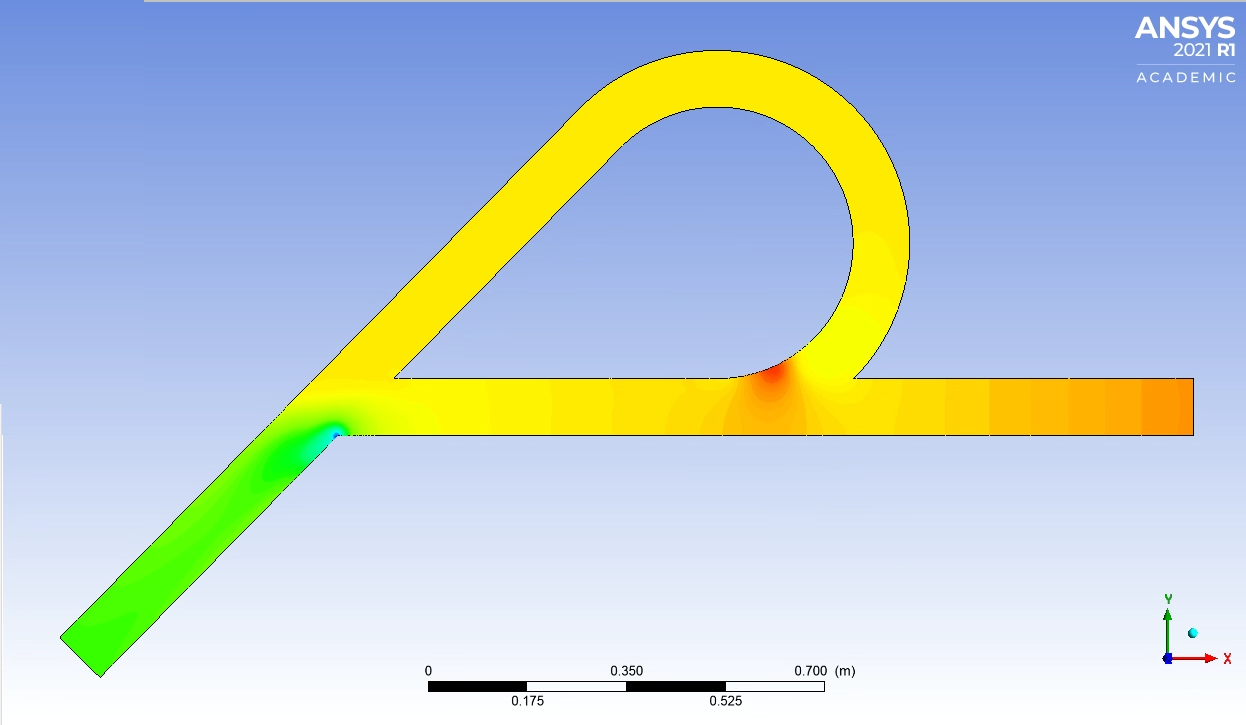
\includegraphics[width=.7\textwidth]{images/task3/sketch.png}
    \caption{Geometry for Task 3}
    \label{fig:task3sketch}
\end{figure}

A mesh size of $5x10^{-3}$ with 300.000+ elements and nodes since ANSYS Student version cannot handle any finer mesh than that value for this case. The necessary plots are given on Figure \ref{fig:omega_epsilon}. It should be noted that while the $k - \omega$ solver struggled highly with the calculations, needing more than 3 times the iterations that $k- \epsilon$ needed. Also, when a reversed flow on a face has occurred, it was seen that the $k - \omega$ solver started to struggle especially, failing to converge properly. \\

When the two models are compared, it can be clearly seen that $k - \omega$ solver has computed more intuitive values especially near the walls as excepted. Since it does not need damping functions like its alternative, it does not inherit their drawbacks, causing in less inaccuracy. The $k - \omega$ solver has shown greater values of pressure near the walls and the areas where this low pressures occur are more continuous and show a more gradient fashion instead of sharply cut sections like $k - \epsilon$ shows. It is likely due to this reason that for most of the geometry, the $k - \epsilon$ solver has calculated higher values of velocity around the valvular conduit whereas its alternative resulted in slightly lower magnitudes of velocity. However, their calculated diodicities are highly in agreement. Table \ref{} shows their resulting diodicity values.\\

\begin{table}[H]
\centering
\caption{Comparison of Diodicities}
\label{tab:compared_diodicities}
\resizebox{.4\textwidth}{!}{%
\begin{tabular}{l|ll}
Solver Type & $k - \omega$ & $k - \epsilon$ \\ \hline
Diodicity   & 2.66         & 2.60          
\end{tabular}%
}
\end{table}

As expected, these values are higher than any other diodicity calculated for this project since we have optimized many dimensions accordingly. Also, the turbulent behavior of flow in this configuration helps with more aggressive drops and changes throughout the valve.

\begin{figure}[H]
 \centering
\begin{subfigure}{.45\textwidth}
  \centering
  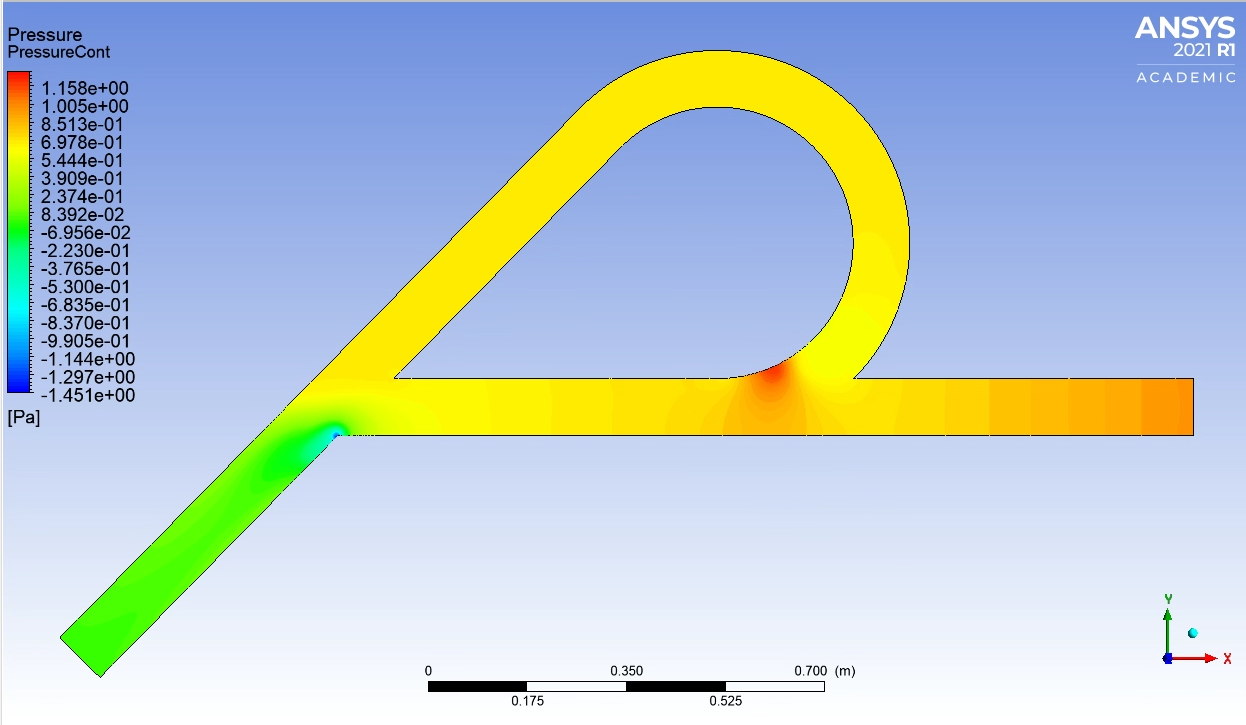
\includegraphics[width=.94\linewidth]{images/task3/epsilon_forward_pressure.png}
  \caption{$k-\epsilon$ Forward Flow Pressure Contours}
  \label{fig:x_d_norm}
\end{subfigure}%
~
\begin{subfigure}{.45\textwidth}
  \centering
  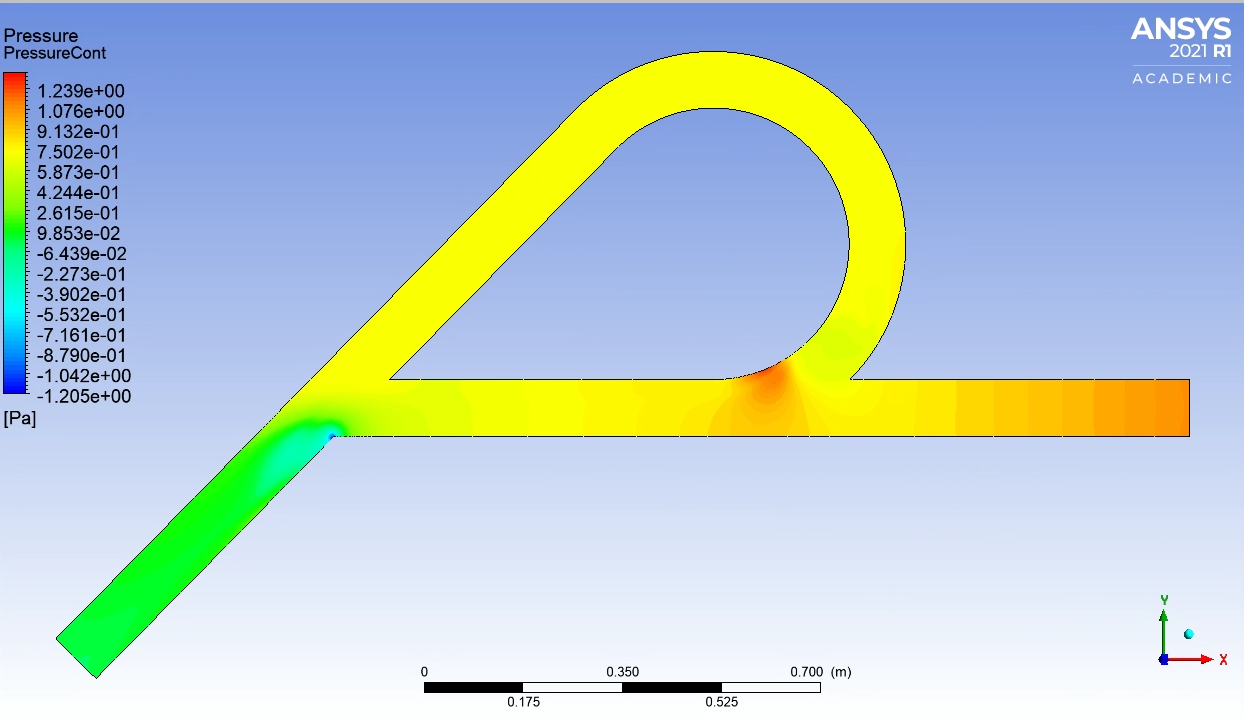
\includegraphics[width=.94\linewidth]{images/task3/omega_forward_pressure.png}
  \caption{$k-\omega$ Forward Flow Pressure Contours}
  \label{fig:x_d_norm_actual}
\end{subfigure}
~
\begin{subfigure}{.45\textwidth}
  \centering
  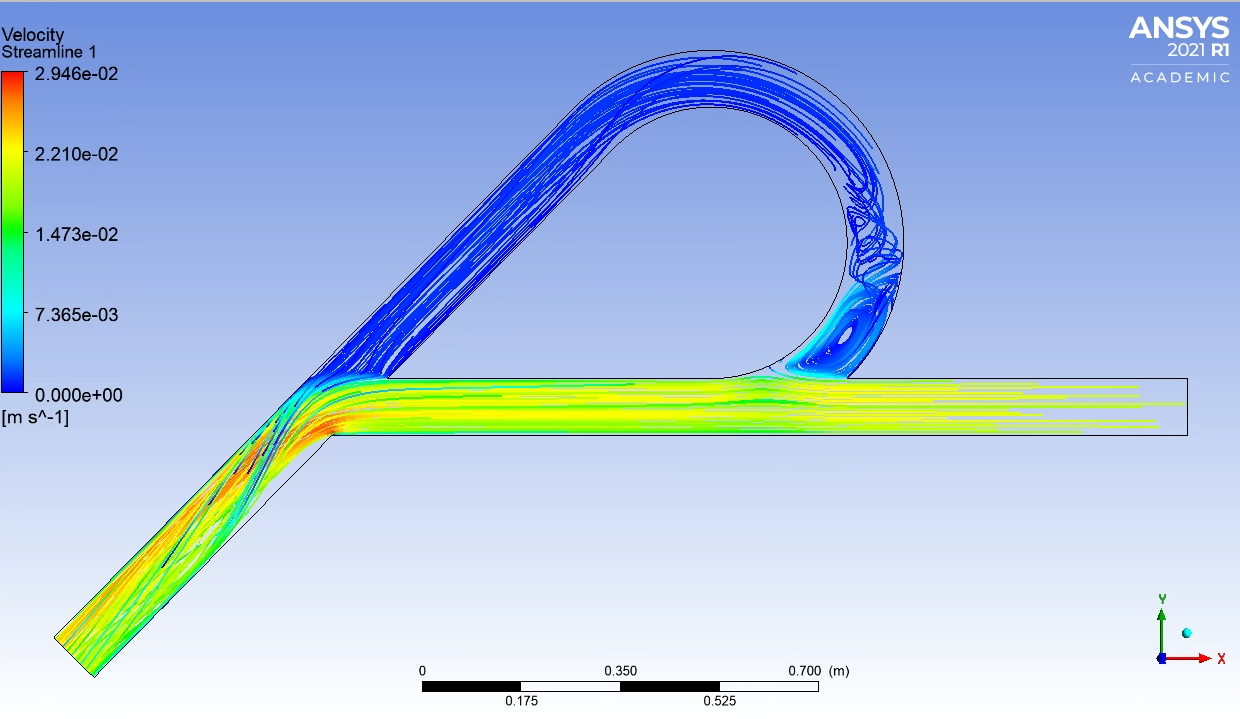
\includegraphics[width=.94\linewidth]{images/task3/epsilon_forward_streamline.png}
  \caption{$k-\epsilon$ Forward Flow Streamlines}
  \label{fig:x_d_norm}
\end{subfigure}%
~
\begin{subfigure}{.45\textwidth}
  \centering
  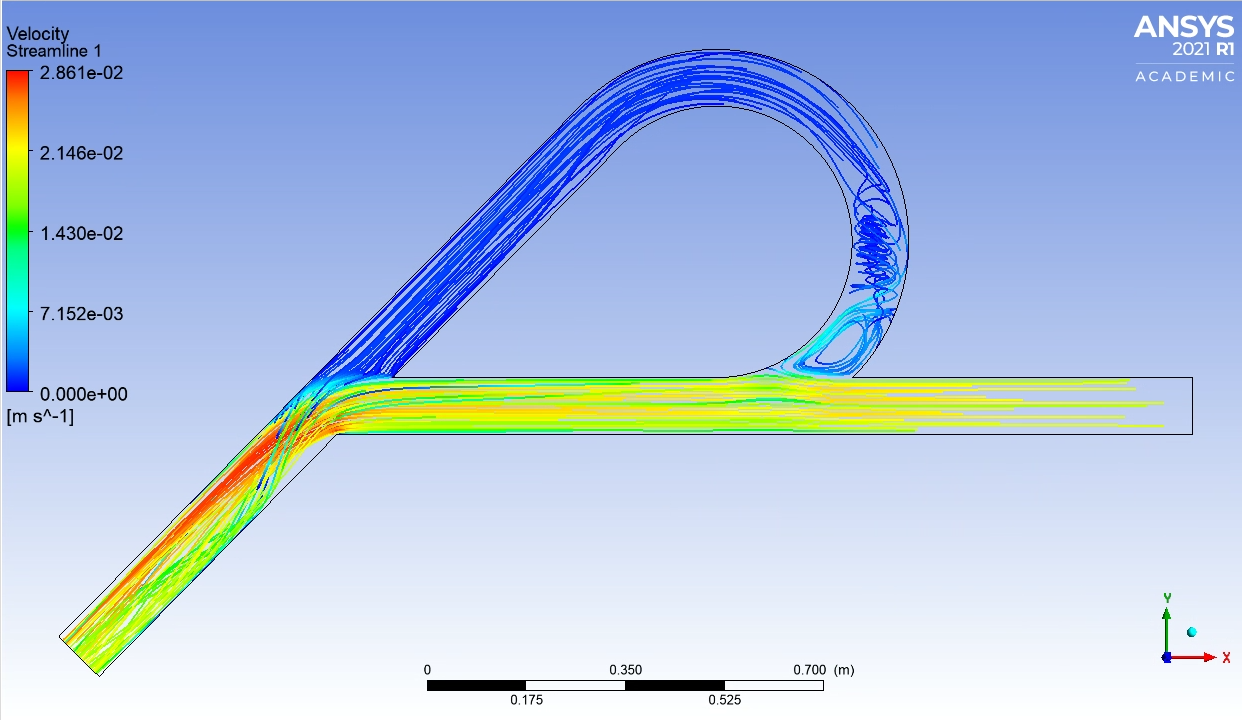
\includegraphics[width=.94\linewidth]{images/task3/omega_forward_streamline.png}
  \caption{$k-\omega$ Forward Flow Streamlines}
  \label{fig:x_d_norm_actual}
\end{subfigure}
~
\begin{subfigure}{.45\textwidth}
  \centering
  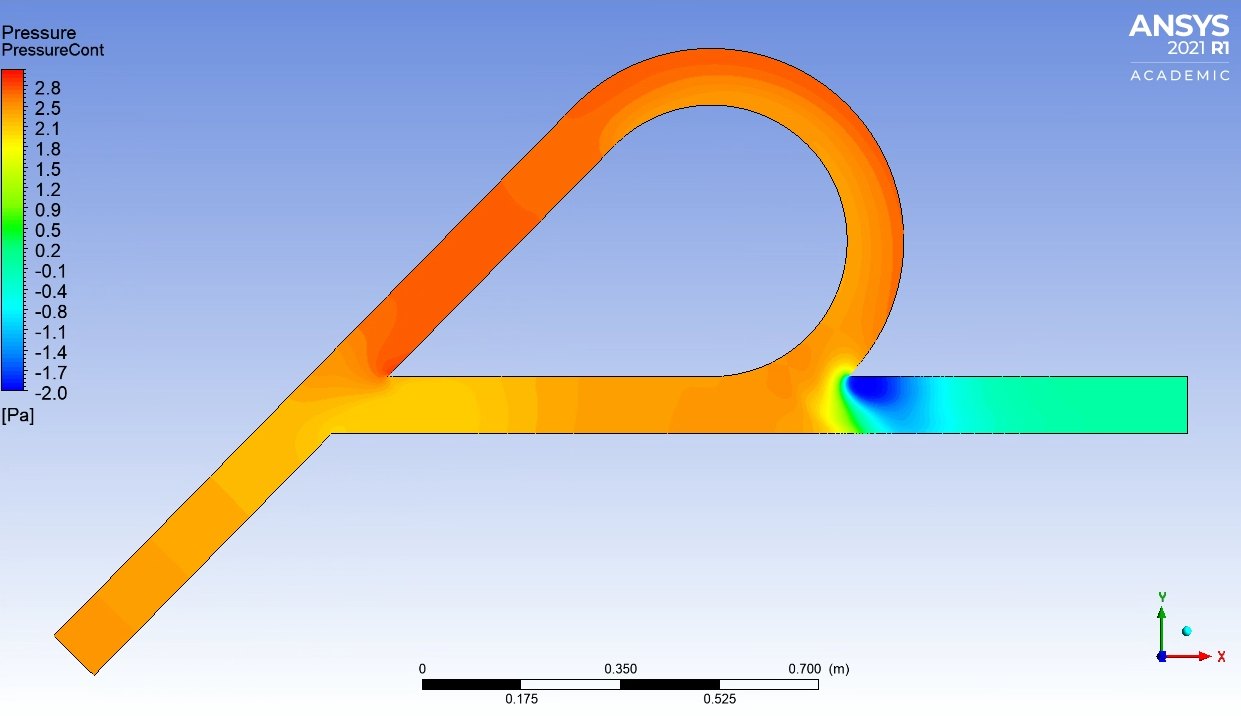
\includegraphics[width=.94\linewidth]{images/task3/epsilon_reverse_pressure.png}
  \caption{$k-\epsilon$ Backward Flow Pressure Contours}
  \label{fig:x_d_norm}
\end{subfigure}%
~
\begin{subfigure}{.45\textwidth}
  \centering
  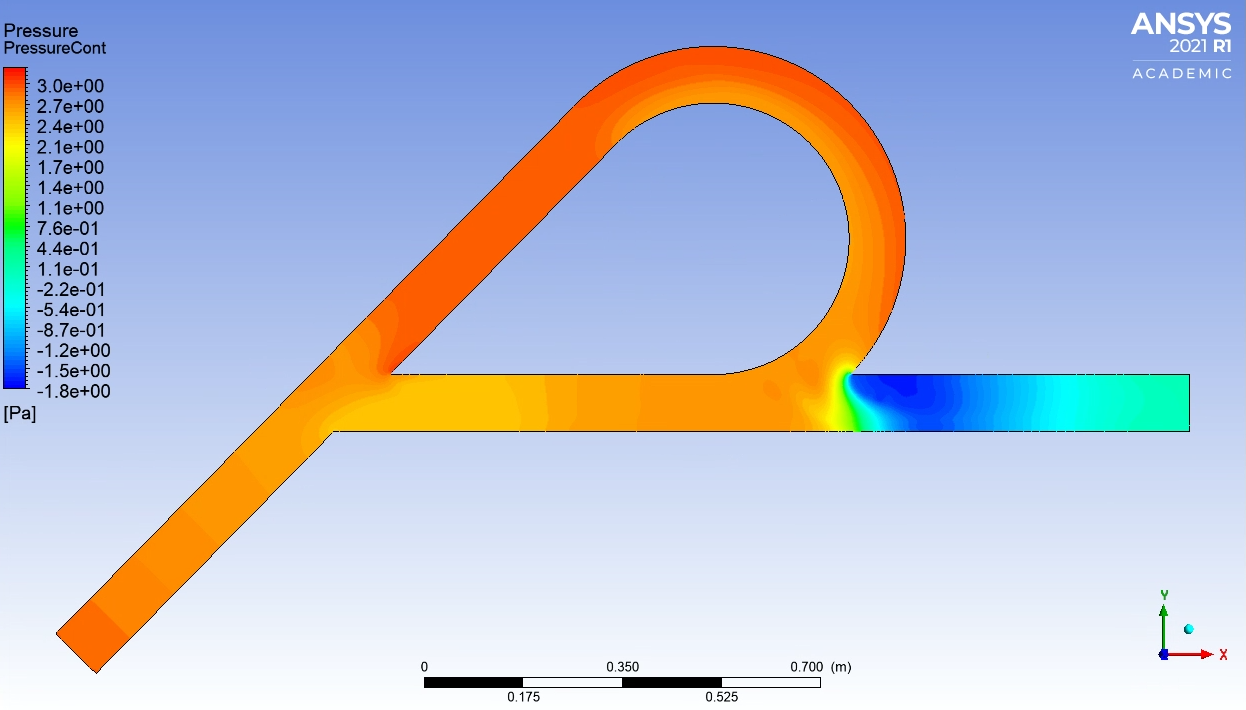
\includegraphics[width=.94\linewidth]{images/task3/omega_backward_pressure.png}
  \caption{$k-\omega$ Backward Flow Pressure Contours}
  \label{fig:x_d_norm_actual}
\end{subfigure}
~
\begin{subfigure}{.45\textwidth}
  \centering
  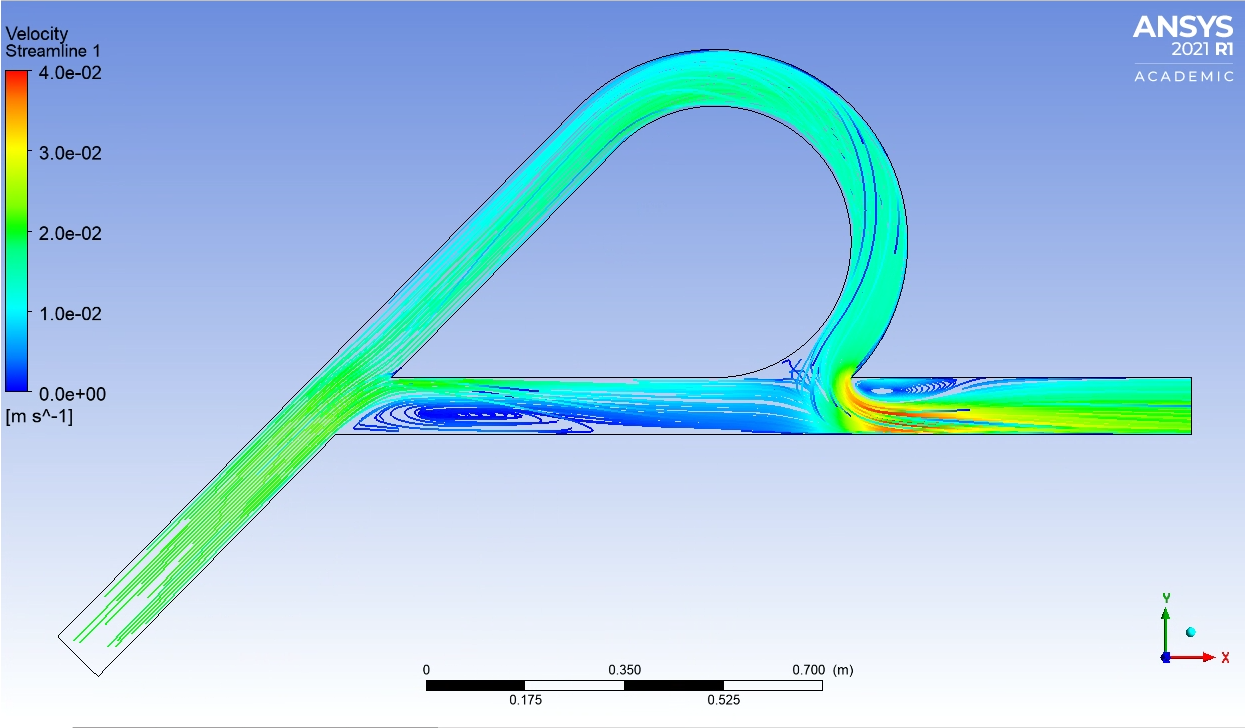
\includegraphics[width=.94\linewidth]{images/task3/epsilon_reverse_streamline.png}
  \caption{$k-\epsilon$ Backward Flow Streamlines}
  \label{fig:x_d_norm}
\end{subfigure}%
~
\begin{subfigure}{.45\textwidth}
  \centering
  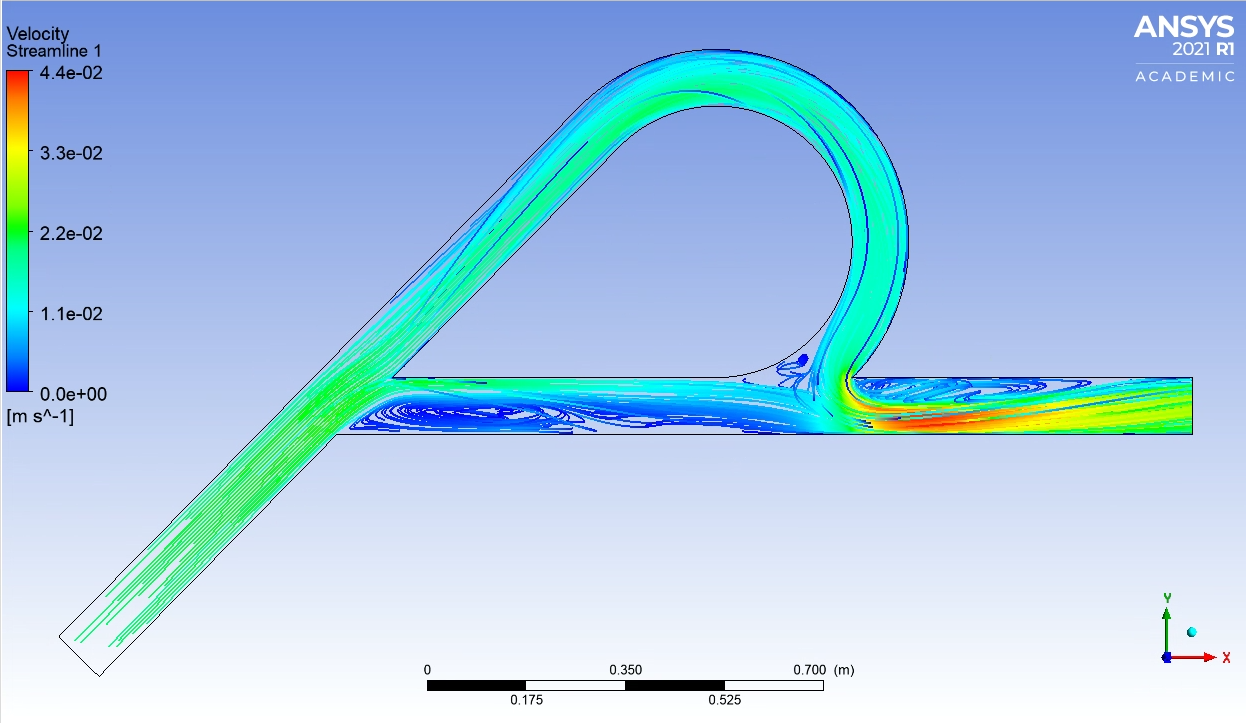
\includegraphics[width=.94\linewidth]{images/task3/omega_backward_streamline.png}
  \caption{$k-\omega$ Backward Flow Streamlines}
  \label{fig:x_d_norm_actual}
\end{subfigure}
~
\caption{Comparison of Turbulence Models}
\label{fig:omega_epsilon}
\end{figure}


%%%%%%%%%%%%%%%%%%%% Conclusion %%%%%%%%%%%%%%%%%%%%%
\section{Conclusion}

In this report many different properties and behaviors of fluid flow through a diodic Tesla valve is 
studied. The flow is simulated for both laminar and turbulent behaviors and valve geometries and types are analyzed and interpreted. Lastly, an optimized straight segment length for the valvular conduit has 
been found and tested. It has been observed that this valve does show significantly diodic behavior without the need of an external energy source or any moving parts. \\ 

While the first task studied the velocity profiles at the inlet and outlets and comparing the with the analytical solution, Couette solution, it has also demonstrated the development of the boundary layer throughout the straight line segments at the inlets and outlets. \\


Although it took some time, the optimization of the straight line segment was quite similar to what Truong et al. reported in their study \cite{truong}. Furthermore, seeing that L value actually delivering the highest diodicity observed among all 18+ simulations made was surely reassuring. \\

Lastly, the same geometry was tested in three dimensions for the first time and turbulence models were used for this task. The results of the models were compared and the necessary plots like the pressure contours and streamlines are utilized to help with the discussion of the results.


\printbibliography
\end{document}